\documentclass[11pt,a4paper]{article}
\usepackage[T1]{fontenc}
\usepackage{lmodern}
\usepackage{babel}
\babelprovide[main,import]{french}
\usepackage{microtype}
\usepackage[a4paper,top=22mm,bottom=21mm,left=24mm,right=24mm,headheight=22pt]{geometry}
\usepackage{amsmath,amssymb,amsthm,mathtools}
\usepackage{graphicx,booktabs,tabularx,array,float}
\usepackage[font=small,labelfont=bf,skip=5pt,labelsep=period]{caption}
\usepackage{tikz}
\usetikzlibrary{arrows.meta,positioning,calc}
\usepackage{tcolorbox}
\tcbuselibrary{breakable,skins}
\usepackage{titlesec,fancyhdr,enumitem,xurl,hyperref}
\definecolor{ink}{HTML}{142639}
\definecolor{teal}{HTML}{087F79}
\definecolor{muted}{HTML}{4A6173}
\definecolor{pale}{HTML}{ECF6F4}
\definecolor{rulecolor}{HTML}{B5CED0}
\definecolor{rust}{HTML}{A14B31}
\hypersetup{colorlinks=true,linkcolor=teal,citecolor=teal,urlcolor=teal,
 pdftitle={Jauge, holonomie et arbitrage sur un réseau de devises},
 pdfsubject={Projet de mathématiques pour la physique},bookmarksdepth=2}
\urlstyle{same}
\setlength{\parindent}{0pt}
\setlength{\parskip}{4.2pt plus 1pt}
\setlength{\emergencystretch}{2em}
\setlength{\textfloatsep}{10pt}
\setcounter{tocdepth}{1}
\captionsetup[table]{name=Tableau}
\renewcommand{\arraystretch}{1.17}
\setlist{leftmargin=*,topsep=2.5pt,itemsep=2.5pt,parsep=0pt}
\titleformat{\part}[display]{\sffamily\bfseries\color{ink}\huge}
  {\normalsize\color{teal}\MakeUppercase{Partie~\thepart}}{4pt}{}
\titlespacing*{\part}{0pt}{0pt}{7pt}
\titleformat{\section}{\sffamily\Large\bfseries\color{ink}}
  {\textcolor{teal}{\thesection}}{0.75em}{}
\titleformat{\subsection}{\sffamily\large\bfseries\color{ink}}
  {\textcolor{teal}{\thesubsection}}{0.75em}{}
\titlespacing*{\section}{0pt}{12pt plus 2pt}{4pt}
\titlespacing*{\subsection}{0pt}{8pt plus 2pt}{2pt}
\pagestyle{fancy}
\fancyhf{}
\fancyhead[L]{\footnotesize\sffamily\color{muted} SUJET MATHÉMATIQUE EN PHYSIQUE}
\fancyhead[R]{\footnotesize\sffamily\color{muted} JAUGE ET ARBITRAGE}
\fancyfoot[R]{\footnotesize\sffamily\color{muted}\thepage}
\renewcommand{\headrulewidth}{0.35pt}
\renewcommand{\headrule}{\hbox to\headwidth{\color{rulecolor}\leaders\hrule height \headrulewidth\hfill}}
\fancypagestyle{plain}{\fancyhf{}\fancyfoot[R]{\footnotesize\sffamily\color{muted}\thepage}\renewcommand{\headrulewidth}{0pt}}
\newtheoremstyle{clair}{5pt}{4pt}{\normalfont}{}{\sffamily\bfseries\color{teal}}{.}{0.5em}{}
\theoremstyle{clair}
\newtheorem{proposition}{Proposition}[section]
\newtheorem{corollaire}[proposition]{Corollaire}
\AtBeginDocument{\renewcommand{\proofname}{Démonstration}}
\newtcolorbox{callout}[1]{enhanced,breakable,colback=pale,colframe=teal,boxrule=0pt,
 borderline west={1.8pt}{0pt}{teal},sharp corners,
 colbacktitle=pale,coltitle=ink,fonttitle=\bfseries\sffamily,
 title={#1},left=3mm,right=3mm,top=0.6mm,bottom=1.5mm,toptitle=1.5mm,bottomtitle=0.5mm}
\newcommand{\R}{\mathbb{R}}
\newcommand{\dd}{\mathrm{d}}
\newcommand{\pb}{\,\mathrm{pb}}
\newcommand{\arrowfx}{\mathbin{\to}}
\newcommand{\filepath}[1]{\nolinkurl{#1}}
\newcommand{\navline}[2]{\hyperref[#2]{#1}\hfill\pageref{#2}\par}
\newcolumntype{Y}{>{\raggedright\arraybackslash}X}
\newsavebox{\plotbox}
\providecommand{\mathdefault}[1]{#1}
\graphicspath{{figures/}}
% Généré par make_report.py depuis les résultats de l'analyse.
\newcommand{\TotalGrille}{240\,000}
\newcommand{\TotalCommuns}{235\,308}
\newcommand{\TotalEligibles}{20\,073}
\newcommand{\TicksSource}{154\,096}
\newcommand{\JuinMarge}{0,182}
\newcommand{\JuilletGrille}{120\,000}
\newcommand{\JuilletEligibles}{6\,733}
\newcommand{\JuilletEligiblesPct}{5,6}
\newcommand{\JuilletMed}{6\,733}
\newcommand{\JuilletNet}{757}
\newcommand{\JuilletNetPct}{11,24}
\newcommand{\JuilletCommun}{116\,407}
\newcommand{\JuilletCommunNet}{19\,742}
\newcommand{\JuilletCommunPct}{16,96}
\newcommand{\JuilletEpisodes}{174}
\newcommand{\JuilletPicDeuxJours}{755}
\newcommand{\JuilletMarge}{0,093}
\newcommand{\JuilletGainPic}{0,279}
\newcommand{\JuilletPicHeure}{12:39:44,100}
\newcommand{\JuilletPicAge}{912}
\newcommand{\JuilletFeeCinq}{81}
\newcommand{\JuilletFeeDix}{0}
\newcommand{\KarpErreur}{\ensuremath{3{,}52\times 10^{-12}}}
\newcommand{\JaugeErreur}{\ensuremath{1{,}24\times 10^{-14}}}
\newcommand{\DualErreur}{\ensuremath{8{,}88\times 10^{-16}}}
\newcommand{\DilatationErreur}{\ensuremath{8{,}88\times 10^{-16}}}
\newcommand{\HodgeJuilletMed}{0,048}
\newcommand{\HodgeJuilletMedPositifs}{0,132}
\newcommand{\HodgeJuilletNonPositifs}{5\,976}
\newcommand{\HodgeJuilletNonPositifsForts}{574}
\newcommand{\DilatationJuilletMed}{0,237}
\newcommand{\DilatationJuilletMax}{1,940}
\newcommand{\ReplayCentOk}{512}
\newcommand{\ReplayCentEval}{608}
\newcommand{\ReplayCentPartInitiale}{67,6}
\newcommand{\ReplayCentPairesOk}{96,87}
\newcommand{\ReplayCentAlertesCouv}{96,43}
\newcommand{\ReplayCentStrictOk}{70}
\newcommand{\ReplayCentStrictTotal}{102}
\newcommand{\ReplayCinqCentsOk}{93}
\newcommand{\ReplayCinqCentsEval}{163}
\newcommand{\ReplayCinqCentsPartInitiale}{12,3}
\newcommand{\RayonCentMin}{0,356}
\newcommand{\RayonCentMax}{0,550}
\newcommand{\RetardCohorte}{6\,721}
\newcommand{\RetardReelCinqCents}{295}
\newcommand{\RetardReelCinqCentsFiltre}{128}
\newcommand{\RetardReelCinqCentsDisparues}{122}
\newcommand{\RetardNulCinqCents}{109}
\newcommand{\RetardNulCinqCentsFiltre}{46}
\newcommand{\RetardNulCinqSecs}{714}
\newcommand{\RetardNulCinqSecsPct}{10,62}
\newcommand{\RetardReelCinqSecs}{1\,074}

\newcommand{\ExpUnCycles}{68}
\newcommand{\ExpUnGrille}{19\,481}
\newcommand{\ExpUnPositifs}{8\,160}
\newcommand{\ExpUnJauge}{\ensuremath{1{,}14\times10^{-13}}}
\newcommand{\ExpTroisErreurJauge}{\ensuremath{2{,}31\times10^{-14}}}
\newcommand{\ExpTroisRepliques}{40}


\begin{document}
\thispagestyle{plain}
{\sffamily\bfseries\small\color{teal} NOTE DE PROJET \hfill NOVEMBRE 2026}

\vspace{12mm}
{\sffamily\bfseries\color{ink}\fontsize{34}{37}\selectfont
 Jauge, holonomie et arbitrage\\[1mm] sur un réseau de devises\par}
\vspace{3mm}
{\sffamily\Large\color{muted} Des connexions sur les fibrés aux cotations bid--ask\par}
\vspace{6mm}
\textcolor{rulecolor}{\rule{\textwidth}{0.7pt}}

\vspace{3mm}
\begin{minipage}[c]{0.61\textwidth}
\textbf{Résumé.} Une connexion peut être plate et conserver une holonomie globale. Nous établissons ce fait sur un fibré en droites, puis passons des formes différentielles aux cochaînes du réseau de devises. Avec un spread, la condition financière devient la recherche d'un potentiel commun compatible avec les fourchettes. Un contre-exemple à quatre devises montre les limites d'un test triangulaire. Trois expériences complètent l'étude des cotations historiques. Un cylindre contrôlé isole une période harmonique, un certificat par cycles mesure la robustesse temporelle et un marché martingale permet de suivre les alertes créées par les retards.
\end{minipage}\hfill
\begin{minipage}[c]{0.34\textwidth}
\centering
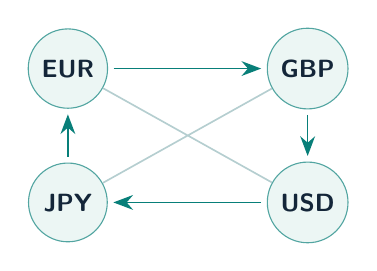
\begin{tikzpicture}[x=1.45cm,y=0.85cm,
  fx/.style={circle,draw=teal!70,fill=pale,minimum size=10mm,font=\small\sffamily\bfseries,text=ink},
  ed/.style={-{Stealth[length=2.5mm]},semithick,draw=teal,shorten >=2pt,shorten <=2pt}]
 \node[fx] (a) at (0,1) {EUR};
 \node[fx] (b) at (2.1,1) {GBP};
 \node[fx] (c) at (2.1,-1) {USD};
 \node[fx] (d) at (0,-1) {JPY};
 \draw[rulecolor,semithick] (a)--(c) (b)--(d);
 \draw[ed] (a)--(b); \draw[ed] (b)--(c);
 \draw[ed] (c)--(d); \draw[ed] (d)--(a);
\end{tikzpicture}
\end{minipage}

\vspace{4mm}
\begin{callout}{Périmètre de l'expérience}
Six paires spot, dix fenêtres de quarante minutes, \TotalGrille{} instants sur une grille de 100~ms. Les données de juin 2024 servent à la calibration. Celles de juillet servent à l'évaluation et au rejeu. La mesure porte sur des cotations affichées et leurs horodatages.
\end{callout}
\vspace{2mm}
\section*{Sommaire}
\begin{minipage}[t]{0.46\textwidth}
\small
\textbf{I\quad Cadre mathématique et état de l'art}\par
\navline{1\quad Fibrés et holonomie}{sec:geometrie}
\navline{2\quad Cochaînes et décomposition de Hodge}{sec:discret}
\navline{3\quad Critères d'arbitrage}{sec:criteres}
\navline{4\quad État de l'art}{sec:etatart}
\navline{Références}{sec:references}
\end{minipage}\hfill
\begin{minipage}[t]{0.48\textwidth}
\small
\textbf{II\quad Dépassement}\par
\navline{5\quad Contre-exemple à quatre devises}{sec:contrex}
\navline{6\quad Marge et robustesse}{sec:marge}
\navline{7\quad Protocole empirique}{sec:protocole}
\navline{8\quad Résultats}{sec:resultats}
\navline{12\quad Conclusion}{sec:conclusion}
\end{minipage}
\vspace{4mm}
{\small
\textbf{III--V\quad Trois expériences géométriques}\par
\navline{Expérience 1\quad Holonomie sur le cylindre}{sec:experience-un}
\navline{Expérience 2\quad Certificats sur les circulations HistData}{sec:experience-deux}
\navline{Expérience 3\quad Transport temporel et retards}{sec:experience-trois}
}
\clearpage

\part{Cadre mathématique et état de l'art}
\label{part:etat}
\section{Fibrés, connexions et holonomie}
\label{sec:geometrie}
\subsection{Du changement d'unités au transport parallèle}

Soit \(M\) une variété lisse connexe et \(L\to M\) un fibré en droites réelles orientées. La fibre \(L_x\) contient les quantités exprimées au point \(x\). Ses repères positifs forment la fibre d'un fibré principal de groupe de Lie \(G=\R_{>0}\), isomorphe à \((\R,+)\) par le logarithme. Sur une variété lisse paracompacte, une partition de l'unité recolle les sections locales positives en une section globale positive. Le fibré est ainsi trivialisable, et le choix de trivialisation fixe les unités.

Dans un repère global, une connexion s'écrit \(\nabla=\dd-A\) avec \(A\in\Omega^1(M)\). Pour une courbe \(\gamma\colon[0,1]\to M\), la condition \(\nabla_{\dot\gamma}u=0\) impose \(\dot u=A_{\gamma}(\dot\gamma)u\). On en déduit le transport entre les deux fibres et sa loi sous le changement de coordonnées \(u'(x)=g(x)u(x)\), \(g=e^\chi>0\).
\begin{equation}
 T_\gamma=\exp\!\left(\int_\gamma A\right),\qquad
 A'=A+\dd\chi,\qquad
 T'_\gamma=g\bigl(\gamma(1)\bigr)\,T_\gamma\,g\bigl(\gamma(0)\bigr)^{-1}.
 \label{eq:continu}
\end{equation}
Les transports se multiplient à la concaténation. Inverser le chemin inverse le transport. Pour un lacet \(C\), l'holonomie \(H(C)=\exp(\oint_C A)\) est invariante par changement de repère. Cette construction reprend la condition de dérivée covariante nulle étudiée pour le transport parallèle dans le cours.

\subsection{Courbure et théorème de Stokes}

On note \(F=\dd A\) la 2-forme de courbure dans la convention du transport \eqref{eq:continu}. Avec \(\nabla=\dd-A\), l'opérateur de courbure agit comme \(-F\) sur la droite. Pour une 2-chaîne orientée \(\Sigma\) de bord \(C\), Stokes donne
\begin{equation}
 \log H(C)=\int_C A=\int_\Sigma F.
 \label{eq:stokes}
\end{equation}
Ainsi la circulation sur une petite plaquette mesure le flux local de \(F\). Dans une carte, \(A=A_\mu\,\dd x^\mu\) et \(F_{\mu\nu}=\partial_\mu A_\nu-\partial_\nu A_\mu\). Le crochet de Lie disparaît parce que \(G\) est abélien \cite{nakahara,tong}.

Pour la connexion électromagnétique de groupe \(U(1)\), le facteur associé à \(C\) prend la forme \(\exp(\mathrm{i}q\oint_C A/\hbar)\). C'est le cas abélien d'une boucle de Wilson. Le pendule de Foucault, étudié en cours, donne un autre exemple de transport dont le résultat dépend du chemin fermé. L'observable y est une rotation du plan tangent. Ici, l'observable est un facteur de changement d'échelle.

\clearpage
\subsection{Platitude locale, périodes et potentiel global}

\begin{proposition}[Obstruction cohomologique]
\label{prop:periods}
Pour une connexion positive sur \(M\) de courbure nulle, les classes de jauge des formes \(A\) sont les éléments de
\[
 H^1_{\mathrm{dR}}(M)
 = \frac{\ker(\dd\colon\Omega^1(M)\to\Omega^2(M))}
        {\operatorname{im}(\dd\colon\Omega^0(M)\to\Omega^1(M))}.
\]
L'holonomie définit alors un homomorphisme \(\pi_1(M,x_0)\to\R_{>0}\). Elle vaut \(1\) sur tous les lacets si et seulement si \(A=\dd\phi\) pour une fonction globale \(\phi\). En particulier, toute connexion positive plate sur une base simplement connexe admet un tel potentiel.
\end{proposition}

\begin{proof}
La loi de jauge \eqref{eq:continu} ajoute exactement une forme exacte. Si \(F=0\), Stokes appliqué à une homotopie de lacets préserve l'intégrale de \(A\), et la concaténation additionne les périodes. Le logarithme du facteur de retour est donc un caractère additif réel. Si chaque période est nulle, l'intégrale \(\phi(x)=\int_{x_0}^x A\) est indépendante du chemin. En prolongeant le chemin dans une carte, on obtient \(\dd\phi=A\). Une forme exacte donne réciproquement des intégrales nulles sur tous les lacets.
\end{proof}

\begin{minipage}[c]{0.62\linewidth}
\textbf{Exemple sur le cylindre.} Sur \(M=S^1\times(0,1)\), notons \(\dd\theta\) la 1-forme angulaire globale, dont l'intégrale sur un tour vaut \(2\pi\). Pour \(A=\frac{\kappa}{2\pi}\dd\theta\), on a \(F=0\). Pourtant, un tour positif donne \(\oint_C A=\kappa\) et \(H(C)=e^\kappa\). Pour \(\kappa\ne0\), \(A\) est fermée et sa classe de de Rham est non nulle \cite{botttu,nakahara}. Le lacet \(C\) entoure le trou et représente un générateur de \(H_1(M;\R)\).
\end{minipage}\hfill
\begin{minipage}[c]{0.34\linewidth}
\centering
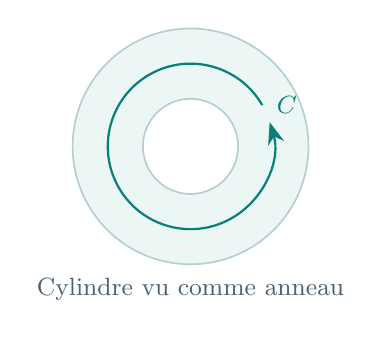
\begin{tikzpicture}[scale=0.93]
 \fill[pale] (0,0) circle (1.61);
 \fill[white] (0,0) circle (0.65);
 \draw[rulecolor,semithick] (0,0) circle (1.61) (0,0) circle (0.65);
 \draw[teal,thick,-{Stealth[length=2.8mm]}] (30:1.13) arc (30:377:1.13);
 \node[font=\small,text=teal] at (23:1.43) {\(C\)};
 \node[font=\small,text=muted] at (0,-1.95) {Cylindre vu comme anneau};
\end{tikzpicture}
\end{minipage}

\begin{callout}{Quelle topologie intervient dans le modèle de change ?}
Le groupe \(\R_{>0}\) est contractile et la droite orientée admet un repère global. L'obstruction provient ici des périodes de la connexion sur la base. La fibration de Hopf étudiée en cours illustre une autre situation, avec un fibré principal \(U(1)\) non trivial. L'effet Aharonov--Bohm fournit l'analogie locale et globale du cylindre, avec une phase là où le modèle de change donne un facteur positif.
\end{callout}

\clearpage
\section{Des formes différentielles aux cochaînes du réseau}
\label{sec:discret}
\subsection{Discrétisation compatible avec Stokes}

Munissons un réseau de sommets, d'arêtes et de faces orientées. Cet ensemble forme un complexe cellulaire \(K\). Une \(p\)-cochaîne assigne un nombre à chaque cellule de dimension \(p\), en changeant de signe quand on renverse l'orientation d'une arête ou d'une face. Les cobords de degré \(0\) et \(1\) s'écrivent
\[
 (d_0h)_{ij}=h_j-h_i,\qquad
 (d_1a)_P=\sum_{e\in\partial P}a_e,\qquad d_1d_0=0.
\]
Dans un maillage d'une variété, l'application \(I\) intègre les formes sur les cellules et évalue les fonctions aux sommets. Elle vérifie \(d_K I=I\dd\) par Stokes. En particulier, les log-transports \(a_e=\int_e A\) changent par \(d_0I(\chi)\) et la circulation sur une face vaut \(\int_P F\). Pour le marché, \(K\) est construit directement à partir des paires cotées. Le modèle s'applique sans coordonnées continues pour les devises.

Dans une connexion réversible sur \(K\), chaque devise \(i\) porte sa droite \(L_i\), chaque lien \(i\arrowfx j\) son facteur de transport \(r_{ij}>0\) et le retour le facteur \(r_{ij}^{-1}\). L'analogue discret de \eqref{eq:continu} est
\begin{equation}
 r'_{ij}=\frac{g_j}{g_i}r_{ij},\qquad a'_{ij}=a_{ij}+\chi_j-\chi_i,\qquad
 a_{ij}=\log r_{ij},\quad \chi_i=\log g_i .
 \label{eq:gauge}
\end{equation}
Pour un cycle \(C=(i_0,\ldots,i_k=i_0)\), le produit des transports et son logarithme sont
\begin{equation}
 H(C)=\prod_{\ell=0}^{k-1}r_{i_\ell i_{\ell+1}},
 \qquad G(C)=\log H(C)=\sum_{e\in C}a_e .
 \label{eq:holonomy}
\end{equation}
L'annulation des \(\chi_j-\chi_i\) vaut aussi pour des taux dirigés avec coûts. On exprime les petits gains en points de base logarithmiques, en multipliant le log-gain par \(10^4\).

\subsection{Quatre devises, trois cycles indépendants}

Pour une 1-cochaîne fermée, la circulation est une fonction des classes de cycles. En effet, les bords de 2-chaînes ont somme nulle. L'espace des classes de jauge fermées est \(H^1(K;\R)=\ker d_1/\operatorname{im}d_0\). Comme dans la proposition \ref{prop:periods}, l'annulation de toutes les périodes équivaut à \(a=d_0h\). Pour le voir, on fixe une racine et on définit \(h_i\) par la somme des poids sur un chemin vers \(i\). Deux chemins donnent la même somme puisque leur différence est un cycle de période nulle.

Le graphe complet à quatre sommets possède six arêtes et un espace des cycles de dimension \(6-4+1=3\). Fixons une racine \(o\). Les trois triangles qui contiennent \(o\) et une paire d'autres sommets forment une base. En effet, \(a_{oi}+a_{ij}+a_{jo}=0\) donne \(a_{ij}=a_{oj}-a_{oi}\). Si l'on attache les quatre faces triangulaires, \(H^1(K;\R)=0\). L'annulation du flux de chaque triangle suffit alors à imposer un potentiel global. Le même raisonnement sur un anneau maillé laisse une période supplémentaire, celle qui entoure le trou.

\clearpage
\subsection{Décomposition de Hodge et distance au potentiel}
\label{sec:hodge}

Le choix d'un produit scalaire sur les cochaînes permet de distinguer les sources d'une circulation \cite{hodge}. Prenons le produit scalaire euclidien dans les bases des cellules orientées et notons \(D_0,D_1\) les matrices des deux cobords. Toute 1-cochaîne \(m\) se décompose en trois termes orthogonaux
\begin{equation}
 m = D_0h + D_1^{\mathsf T}\beta + \eta,\qquad
 \eta\in\ker D_1\cap\ker D_0^{\mathsf T}.
 \label{eq:hodge}
\end{equation}
Les images de \(D_0\) et \(D_1^{\mathsf T}\) sont orthogonales puisque \(D_1D_0=0\). Leur complément orthogonal commun est l'espace harmonique indiqué dans \eqref{eq:hodge}. Le premier terme est la projection sur les différences de potentiels. Le second porte les défauts de circulation locaux. Le troisième est fermé, peut porter des périodes globales et représente les classes de \(H^1(K;\R)\). En effet, si \(m\) est fermé, il est orthogonal à \(\operatorname{im}D_1^{\mathsf T}\) et son terme harmonique est l'unique représentant orthogonal aux cochaînes exactes.

Dans le complexe à quatre devises avec toutes ses faces triangulaires, \(D_0\) et \(D_1\) ont chacun rang \(3\). L'espace des 1-cochaînes a dimension \(6\), donc \(\eta=0\). Le cylindre maillé fournit un exemple harmonique non nul. Relions deux anneaux de quatre sommets par quatre faces carrées. Donnons le poids \(1/4\) aux arêtes dans le sens de chaque tour et le poids zéro aux arêtes verticales. Les contributions se compensent autour de chaque face et à chaque sommet, donc \(D_1m=D_0^{\mathsf T}m=0\). Chaque tour porte la période \(1\).

Sur les six paires du graphe complet, les matrices vérifient
\begin{equation}
 D_0D_0^{\mathsf T}+D_1^{\mathsf T}D_1=4I_6.
 \label{eq:laplacien}
\end{equation}
Chaque arête a deux extrémités et appartient à deux faces, ce qui donne \(4\) sur la diagonale. Deux arêtes disjointes donnent zéro dans les deux matrices. Deux arêtes adjacentes appartiennent à une face commune, et le signe de leur contribution à la matrice de face est l'opposé du signe donné par leur sommet commun. Ainsi les coefficients hors diagonale s'annulent.

Il en résulte une formule explicite pour le résidu \(R\) de la projection sur les potentiels et sa taille quadratique moyenne \(\sigma_H\).
\begin{equation}
 R=m-D_0\widehat h=\tfrac14D_1^{\mathsf T}D_1m,\qquad
 \sigma_H(m)=\frac{\|R\|_2}{\sqrt{6}} .
 \label{eq:hodge-rms}
\end{equation}
En effet, \(\tfrac14D_0D_0^{\mathsf T}m\) appartient à l'espace des potentiels, et \(\tfrac14D_1^{\mathsf T}D_1m\) est orthogonal à cet espace. Le résidu est invariant sous \(m\mapsto m+D_0\chi\). Le calcul numérique applique \eqref{eq:hodge-rms} aux taux du milieu de la fourchette. La valeur obtenue mesure un défaut géométrique en points de base logarithmiques.

\clearpage
\section{Critères d'arbitrage et cohérence des prix}
\label{sec:criteres}
\subsection{Transport réversible et potentiel global}

Sans coûts, une boucle de facteur différent de \(1\) donne un gain dans l'un des deux sens, car \(H(C^{-1})=H(C)^{-1}\). L'absence de gain cyclique équivaut donc à \(a=d_0h\). Ce critère utilise l'annulation de toutes les périodes de la connexion. Sur le complexe complet de la section \ref{sec:discret}, on peut tester les trois triangles de base.

\subsection{Avec bid--ask, la platitude devient une inégalité}

Une paire $i/j$ est cotée en unités de $j$ par unité de $i$. On reçoit le bid $B_{ij}$ en vendant $i$ et on paie l'ask $A_{ij}$ en l'achetant. Pour $0<B_{ij}\le A_{ij}$,
\begin{equation}
\begin{aligned}
 a_{ij}&=\log B_{ij}=m_{ij}-s_{ij},&
 a_{ji}&=-\log A_{ij}=-m_{ij}-s_{ij},\\
 m_{ij}&=\tfrac12\log(A_{ij}B_{ij}),&
 s_{ij}&=\tfrac12\log(A_{ij}/B_{ij})\ge0.
\end{aligned}
 \label{eq:mid}
\end{equation}
Ici $m$ est le logarithme du milieu géométrique de la fourchette et $s$ le demi-spread logarithmique. Sur une boucle, $G(C)=\sum_{e\in C}m_e-\sum_{e\in C}s_e$, avec $m_{ji}=-m_{ij}$ et $s_{ji}=s_{ij}$. Le spread est invariant par \eqref{eq:gauge}. L'aller-retour vaut $G(i,j,i)=-2s_{ij}$. La partie $m$ constitue la connexion réversible. Les taux exécutables définissent deux liens orientés distincts et leurs coûts s'additionnent le long d'un trajet.

\begin{proposition}[Critère statique avec coûts proportionnels]
\label{prop:static}
Pour un graphe fini de taux instantanément disponibles, les conditions suivantes sont équivalentes.
\begin{enumerate}[label=\textnormal{(\roman*)}]
 \item Tout cycle dirigé vérifie $G(C)\le0$.
 \item Il existe $h\in\R^{V}$ tel que $a_{ij}\le h_j-h_i$ sur chaque arête.
 \item Il existe des valeurs $v_i>0$ telles que $r_{ij}v_j\le v_i$ sur chaque arête.
\end{enumerate}
Dans le cas bid--ask, la dernière condition place le taux implicite $v_i/v_j$ entre $B_{ij}$ et $A_{ij}$.
\end{proposition}

\begin{proof}
Une somme de différences de potentiels est nulle sur un cycle, d'où (ii)$\Rightarrow$(i). Pour (i)$\Rightarrow$(ii), ajoutons une source reliée à chaque sommet par un arc de poids nul. Pour tout sommet $j$, soit $h_j$ le plus grand poids d'un chemin de cette source à $j$. Retirer d'un chemin une boucle de poids non positif ne diminue jamais son poids. On peut donc maximiser parmi un ensemble fini de chemins simples, et $h_j$ est bien défini. Un chemin optimal vers $i$ prolongé par $i\arrowfx j$ donne $h_j\ge h_i+a_{ij}$. Enfin, prendre $v_i=e^{-h_i}$ convertit (ii) en (iii). Appliquer (iii) à l'arête inverse donne la borne supérieure $v_i/v_j\le A_{ij}$.
\end{proof}

Appliquée aux deux directions de chaque paire, la condition (ii) s'écrit
\begin{equation}
 \bigl|m_{ij}-(h_j-h_i)\bigr|\le s_{ij}.
 \label{eq:fourchette}
\end{equation}
Ainsi les fourchettes sont compatibles exactement lorsqu'elles contiennent une 1-cochaîne exacte. La décomposition de Hodge projette le milieu au sens quadratique. L'inégalité \eqref{eq:fourchette} exige que chaque arête respecte sa propre tolérance.

\clearpage
\subsection{Bellman--Ford, portefeuilles et théorème fondamental}

Avec les poids $-a_{ij}$, une boucle profitable est un cycle de poids négatif, le cas d'application classique de Bellman--Ford \cite{sedgewick}. Les relaxations de plus court chemin calculent l'analogue de $-h$ et détectent une amélioration indéfinie liée à un cycle négatif. On peut restreindre la recherche aux cycles simples. Tout parcours fermé avec répétitions se décompose en cycles simples, et une somme positive contient au moins un terme positif. La formulation géométrique et la détection par graphe portent donc sur la même information lorsqu'elles utilisent les mêmes taux dirigés.

La condition (iii) fournit un certificat pour les portefeuilles statiques. Valoriser un portefeuille $x$ par $\sum_i v_i x_i$ donne une fonction qui ne peut pas augmenter au cours d'une conversion aux taux du graphe. À l'inverse, dans le modèle idéal où la devise de départ peut être empruntée puis rendue immédiatement sans frais, un cycle de facteur $H(C)>1$ fournit un surplus certain à capital initial nul. Ces arguments concernent des prix simultanés et des conversions proportionnelles, avec la taille de transaction supposée disponible.

En temps continu, le théorème de Delbaen et Schachermayer relie la condition \emph{No Free Lunch with Vanishing Risk} (NFLVR) à l'existence d'une mesure équivalente de martingale locale pour des prix actualisés localement bornés, sous les hypothèses du théorème \cite{delbaen}. Avec des coûts de transaction et du risque dans le temps, le système de prix cohérent de Schachermayer combine les contraintes du bid--ask avec des propriétés de martingale et des hypothèses d'absence d'arbitrage robuste \cite{schachermayer}. Le changement de numéraire stochastique consiste à choisir un actif de référence positif et, sous les conditions appropriées, à changer de mesure pour préserver la propriété de martingale des prix exprimés dans ce numéraire \cite{geman}. La transformation \eqref{eq:gauge} exprime ici un changement d'unités locales à instant fixé.

\subsection{Un réseau espace-temps pour comparer deux transports}
\label{sec:temps}

On peut attribuer une fibre à chaque sommet \((i,t)\). Un lien de conversion porte le log-taux à l'instant \(t\). Un lien temporel \((i,t)\arrowfx(i,t')\) porte le log-facteur de détention \(b_i(t,t')\). Pour la connexion au milieu des fourchettes, une plaquette compare les deux chemins qui convertissent \(i\) en \(j\) soit avant, soit après la détention.
\begin{equation}
 \mathcal F_{ij;t,t'}
   =m_{ij}(t)+b_j(t,t')-m_{ij}(t')-b_i(t,t').
 \label{eq:espace-temps}
\end{equation}
Chaque chemin relie \((i,t)\) à \((j,t')\). Une jauge \(g_i(t)\) ajoute le même écart de logarithmes aux deux transports. Leur différence \eqref{eq:espace-temps} est donc invariante. La plaquette se lit comme une comparaison de deux chemins orientés vers l'avenir.

\begin{center}
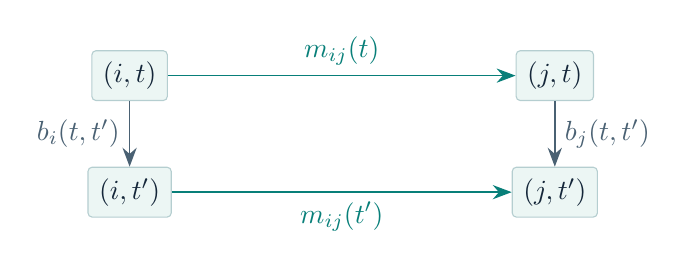
\begin{tikzpicture}[x=1cm,y=1cm,
  state/.style={draw=rulecolor,fill=pale,rounded corners=1.5pt,inner sep=4pt,text=ink},
  timelink/.style={-{Stealth[length=2.4mm]},semithick}]
 \node[state] (i0) at (0,0) {\((i,t)\)};
 \node[state] (j0) at (5.4,0) {\((j,t)\)};
 \node[state] (i1) at (0,-1.48) {\((i,t')\)};
 \node[state] (j1) at (5.4,-1.48) {\((j,t')\)};
 \draw[timelink,teal] (i0) -- node[above] {\(m_{ij}(t)\)} (j0);
 \draw[timelink,teal] (i1) -- node[below] {\(m_{ij}(t')\)} (j1);
 \draw[timelink,muted] (i0) -- node[left] {\(b_i(t,t')\)} (i1);
 \draw[timelink,muted] (j0) -- node[right] {\(b_j(t,t')\)} (j1);
\end{tikzpicture}
\end{center}

Un cycle séquentiel de conversions revient dans la devise \(i\) à un instant ultérieur \(t'\). Le gain de référence compare le transport le long de ce trajet, conversions et détentions comprises, à celui d'un capital détenu en \(i\) de \(t\) à \(t'\). Le rapport est invariant sous \(g_i(t)\) parce que les extrémités coïncident. Le rejeu prend \(b_i(t,t')=0\) dans les unités de cotation pour les délais de quelques secondes étudiés. Ce choix fixe la convention de portage du calcul.

\clearpage
\section{État de l'art et lien avec le cours}
\label{sec:etatart}
\small
\begin{tabularx}{\textwidth}{@{}>{\raggedright\arraybackslash}p{0.29\textwidth}Y@{}}
\toprule
\textbf{Référence} & \textbf{Résultat ou apport pertinent pour le projet}\\
\midrule
Nakahara, Bott et Tu, Jiang et al. \cite{nakahara,botttu,hodge} &
Le transport sur fibré et les périodes des formes fermées structurent la distinction local--global. La théorie de Hodge combinatoire fournit le calcul du défaut au potentiel sur un réseau.\\
Ilinski \cite{ilinski97,ilinski} &
Les échanges et l'actualisation sont interprétés comme transports dans un fibré. Les boucles représentent des opérations financières fermées. Les versions dynamiques ajoutent des hypothèses de modélisation.\\
Sornette \cite{sornette} &
La redérivation de résultats comme Black--Scholes ou la lognormalité apporte peu de validation indépendante. La critique vise aussi les hypothèses dynamiques et la confusion possible entre bruit et gain exploitable.\\
Vazquez et Farinelli \cite{vazquez}, Farinelli et Takada \cite{farinelli} &
Dans des cadres stochastiques spécifiés, les auteurs relient des notions d'arbitrage à des invariants et à la courbure d'une connexion. Le second article examine notamment la condition NUPBR pour une classe de diffusions d'Itô.\\
Aiba et al., Fenn et al., Ito et al. \cite{aiba,fenn,ito} &
Aiba et al. étudient les écarts triangulaires et proposent une dynamique couplée. Fenn et al. observent des écarts brefs et de faible ampleur sur des cotations exécutables. Ito et al. étudient séparément la disponibilité des prix et le risque d'exécution incomplète.\\
Cross et al. \cite{cross}, Cui et Taylor \cite{cui} &
Le premier travail étudie des séquences périodiques d'arbitrages triangulaires entre quatre devises. Le second détecte des cycles à $k$ devises par des produits matriciels max-plus.\\
\bottomrule
\end{tabularx}
\normalsize

Les chapitres du cours sur les connexions, le transport parallèle et l'holonomie mènent à la proposition \ref{prop:periods}. Les formes différentielles, Stokes et la cohomologie de de Rham expliquent le passage de \eqref{eq:stokes} aux circulations de faces. La section \ref{sec:hodge} transpose la décomposition de Hodge aux cochaînes du réseau. Ce cadre sépare deux questions sur les cotations. Quelle est la taille de l'écart à un potentiel global ? Les fourchettes bid--ask suffisent-elles à l'absorber ?

\clearpage
\part{Dépassement et application}
\label{part:dep}
Le travail propre au projet relie la distance au potentiel aux fourchettes observées. Il combine une construction à quatre devises, un certificat sous incertitude et une expérience sur six paires à travers deux périodes distinctes. Les résultats de graphes et de cohomologie fournissent le cadre. L'expérience compare les défauts géométriques aux signaux qui survivent aux coûts, à la fraîcheur et aux délais.

\section{Un cycle profitable malgré tous les triangles déficitaires}
\label{sec:contrex}

Pour le quadrilatère $C=(i,j,k,\ell,i)$, la décomposition en deux triangles fait intervenir deux conversions supplémentaires sur la diagonale $i$--$k$. En additionnant les deux log-gains, on trouve exactement
\begin{equation}
 G(i,j,k,i)+G(i,k,\ell,i)
 =G(i,j,k,\ell,i)+a_{ki}+a_{ik}
 =G(C)-2s_{ik}.
 \label{eq:triangles}
\end{equation}
Dans le cas réversible, le terme supplémentaire s'annule. Avec spread, les deux triangles peuvent être négatifs alors que le tour du quadrilatère est positif. Si tous les triangles sont déficitaires, le gain du quadrilatère est borné par deux fois le demi-spread de chacune de ses diagonales, en appliquant \eqref{eq:triangles} aux deux découpages possibles.

\begin{minipage}[c]{0.48\textwidth}
\centering
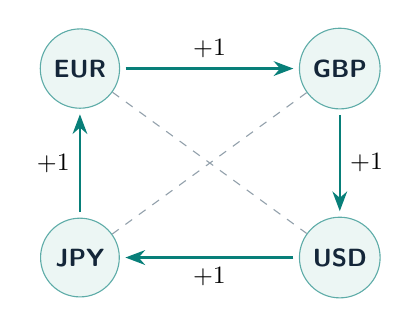
\begin{tikzpicture}[x=1.65cm,y=1.2cm,
  fx/.style={circle,draw=teal!65,fill=pale,minimum size=10mm,font=\small\sffamily\bfseries,text=ink},
  ed/.style={-{Stealth[length=2.5mm]},thick,draw=teal,shorten >=2pt,shorten <=2pt}]
 \node[fx] (a) at (0,1) {EUR};
 \node[fx] (b) at (2.0,1) {GBP};
 \node[fx] (c) at (2.0,-1) {USD};
 \node[fx] (d) at (0,-1) {JPY};
 \draw[dashed,muted!60] (a)--(c) (b)--(d);
 \draw[ed] (a)--node[above,font=\small] {$+1$} (b);
 \draw[ed] (b)--node[right,font=\small] {$+1$} (c);
 \draw[ed] (c)--node[below,font=\small] {$+1$} (d);
 \draw[ed] (d)--node[left,font=\small] {$+1$} (a);
\end{tikzpicture}
\end{minipage}\hfill
\begin{minipage}[c]{0.50\textwidth}
\centering
\small
\begin{tabular}{@{}lrrrr@{}}
\toprule
 & EUR & GBP & USD & JPY\\
\midrule
EUR & -- & $+1$ & $-3$ & $-3$\\
GBP & $-3$ & -- & $+1$ & $-3$\\
USD & $-3$ & $-3$ & -- & $+1$\\
JPY & $+1$ & $-3$ & $-3$ & --\\
\bottomrule
\end{tabular}

\vspace{2mm}
Poids $10^4a_{ij}$ par direction. Chaque ligne indique la devise vendue.
\end{minipage}

\begin{proposition}[Les tests triangulaires peuvent échouer]
Les taux définis par cette matrice ont des spreads bid--ask compatibles. Tous les cycles de longueur deux ou trois sont déficitaires. Le cycle EUR\,$\arrowfx$\,GBP\,$\arrowfx$\,USD\,$\arrowfx$\,JPY\,$\arrowfx$\,EUR gagne quatre points de base logarithmiques.
\end{proposition}
\begin{proof}
Pour toute paire, $a_{ij}+a_{ji}<0$. On peut donc poser $B_{ij}=e^{a_{ij}}$ et $A_{ij}=e^{-a_{ji}}$ dans le sens de cotation choisi, avec $B_{ij}<A_{ij}$. Chaque aller-retour perd au moins deux points de base. Un triangle contient au plus deux arêtes du cycle orienté marqué $+1$ et au moins une arête à $-3$. Son gain vaut au plus $1+1-3=-1\pb$. Le cycle orienté à quatre arêtes réalise $4\pb$, soit $e^{4/10^4}-1$ en rendement simple. Aucun autre cycle n'a de moyenne supérieure à $1\pb$ par arête puisque chaque poids individuel est au plus $1\pb$.
\end{proof}

Un changement d'unités peut rapprocher les taux de l'exemple des niveaux usuels en conservant les spreads relatifs et les gains. Sur le quadrilatère favorable, la période des milieux est de \(8\pb\) et le coût cumulé de \(4\pb\). Leur rapport vaut \(2\) et réalise le maximum de \eqref{eq:dilatation}, car aucun rapport par arête ne dépasse \(2\).

\clearpage
\section{Marge de cycle et certificat sous incertitude}
\label{sec:marge}
\subsection{Le coût critique par conversion}

Soit $q_{ij}>0$ un poids de coût sur chaque arête. Imposer un niveau de frais $\lambda\ge0$ revient à remplacer $a_{ij}$ par $a_{ij}-\lambda q_{ij}$, donc à multiplier $r_{ij}$ par $e^{-\lambda q_{ij}}$. La quantité pertinente pour ce scénario est
\begin{equation}
 \rho_q(a)=\max_{C\ \mathrm{simple}}\frac{\sum_{e\in C}a_e}{\sum_{e\in C}q_e}.
 \label{eq:ratio}
\end{equation}
On suppose ici que le graphe possède au moins un cycle. Pour des coûts identiques sur chaque conversion, $q_e=1$, on note $\mu(a)=\rho_{\boldsymbol{1}}(a)$ la moyenne maximale d'un cycle.

\begin{proposition}[Formulation duale et frais critiques]
\label{prop:dual}
Pour les taux et les poids de coût ci-dessus,
\begin{equation}
 \rho_q(a)=\min_{h\in\R^V}\;\max_{i\arrowfx j}
              \frac{a_{ij}-(h_j-h_i)}{q_{ij}}.
 \label{eq:dual}
\end{equation}
Le plus petit niveau de frais $\lambda\ge0$ qui élimine tout cycle de gain strictement positif est $\max(0,\rho_q(a))$.
\end{proposition}
\begin{proof}
Pour tout $h$, une somme des contraintes $a_{ij}-(h_j-h_i)\le\lambda q_{ij}$ sur un cycle donne $\sum_C a_e\le\lambda\sum_Cq_e$. Tout $\lambda$ admissible est donc supérieur ou égal à $\rho_q(a)$. En sens inverse, pour $\lambda=\rho_q(a)$, les poids $a_{ij}-\lambda q_{ij}$ donnent une somme non positive sur tous les cycles simples, puis sur tous les parcours fermés par décomposition. La proposition \ref{prop:static} donne un potentiel $h$ satisfaisant les contraintes, et le minimum est atteint. Enfin, pour $\lambda<\rho_q(a)$, un cycle qui atteint le maximum dans \eqref{eq:ratio} a un gain strictement positif après frais.
\end{proof}

La moyenne maximale est invariante par changement de jauge. Elle vérifie $\mu(a-c)=\mu(a)-c$ pour tout décalage uniforme $c$ sur les arêtes et $|\mu(a+u)-\mu(a)|\le\max_e|u_e|$. En effet, chaque moyenne de cycle varie d'au plus $\max_e|u_e|$, et la borne se conserve au passage au maximum. Le décalage uniforme montre que la constante de cette borne est optimale.

Sur le graphe de l'expérience, il y a $6$ allers-retours, $8$ triangles orientés et $6$ quadrilatères orientés, à rotation près. L'énumération de ces $20$ cycles donne aussi un témoin. Pour un graphe dirigé fortement connexe à $n$ sommets, l'algorithme de Karp calcule $\mu$ en $O(n|E|)$ \cite{karp}. Avec une racine fixée $o$, on initialise $D_0(o)=0$ et les autres $D_0(v)=-\infty$, puis
\[
 D_k(v)=\max_{u\arrowfx v}\{D_{k-1}(u)+a_{uv}\},
 \qquad
 \mu=\max_{v:D_n(v)>-\infty}\;
      \min_{0\le k<n:\,D_k(v)>-\infty}\frac{D_n(v)-D_k(v)}{n-k}.
\]
C'est la version à poids maximaux du théorème de Karp. Le calcul est confronté à l'énumération et au test de signe de Bellman--Ford.

\subsection{Distance au potentiel mesurée en unités de spread}
\label{sec:dilatation}

On cherche le plus petit facteur \(\Lambda_\star\ge0\) par lequel multiplier tous les demi-spreads pour rendre \eqref{eq:fourchette} réalisable. Pour des spreads strictement positifs, la proposition \ref{prop:dual} appliquée aux poids dirigés \(m_{ij}\) et aux coûts \(s_{ij}\) donne
\begin{equation}
 \Lambda_\star(m,s)
 =\min_h\max_{\{i,j\}}\frac{|m_{ij}-(h_j-h_i)|}{s_{ij}}
 =\max_{C\ \mathrm{simple}}
       \frac{\left|\sum_{e\in C}m_e\right|}{\sum_{e\in C}s_e}.
 \label{eq:dilatation}
\end{equation}
Les valeurs absolues viennent des deux orientations. Si un demi-spread vaut zéro, l'arête correspondante impose l'égalité. La formule par cycles reste valable en prenant \(0/0=0\) et un rapport infini pour une période non nulle sur un cycle de coût nul. En effet, le critère de la proposition \ref{prop:static} revient à imposer \(\big|\sum_C m_e\big|\le\Lambda_\star\sum_C s_e\) sur tous les cycles.

Ce facteur est la distance à l'espace des cochaînes exactes pour la norme uniforme pondérée par \(s\) quand \(s>0\). Il est invariant par jauge. Les fourchettes observées admettent un potentiel si et seulement si \(\Lambda_\star\le1\).

\clearpage
\subsection{Enveloppe de prix et trois décisions possibles}

Au temps de décision, écrivons $a$ pour le graphe nominal et $u_e\ge0$ pour une marge d'incertitude sur chaque log-taux. Si $a_e^\ast$ est le log-taux pertinent pour une conversion, on suppose $a_e-u_e\le a_e^\ast\le a_e+u_e$. Pour une séquence de conversions, cette hypothèse s'applique à chaque arête à son propre temps d'exécution.

\begin{proposition}[Bornes inférieure et supérieure]
\label{prop:robust}
Soient $\mu_-:=\mu(a-u)$ et $\mu_+:=\mu(a+u)$.
\begin{enumerate}
 \item Si $\mu_->0$, un cycle déterminé à partir de $a-u$ reste profitable pour tous les taux compatibles avec les bornes, y compris si ses différentes arêtes sont lues à des instants différents.
 \item Si $\mu_+\le0$, chaque cycle considéré a un gain non positif pour tous les taux compatibles.
 \item Pour un graphe statique et une boîte complète $\prod_e[a_e-u_e,a_e+u_e]$, les deux bornes sont atteintes par des graphes de la boîte. Si $\mu_-\le0<\mu_+$, il existe donc un scénario sans gain et un scénario avec gain.
\end{enumerate}
\end{proposition}
\begin{proof}
Pour tout cycle, la somme des poids évalués est comprise entre $\sum_C(a_e-u_e)$ et $\sum_C(a_e+u_e)$. Si le maximum des moyennes inférieures est positif, le cycle qui atteint ce maximum est le témoin demandé. Si le maximum des moyennes supérieures est non positif, tous les cycles ont une somme supérieure non positive. Dans la boîte statique complète, les deux coins $a-u$ et $a+u$ sont admissibles et atteignent les bornes. Des restrictions supplémentaires, par exemple une dépendance entre bid et ask ou des mouvements communs entre paires, peuvent exclure ces coins et rendre l'enveloppe conservatrice.
\end{proof}

Si tous les $u_e$ sont strictement positifs, $\rho_u(a)$ donne aussi le facteur d'incertitude critique. Sous les chocs défavorables $a-\theta u$, il reste un cycle robuste exactement lorsque $\theta<\rho_u(a)$, pour $\theta\ge0$. La preuve est l'identité
\[
 \sum_{e\in C}(a_e-\theta u_e)>0
 \quad\Longleftrightarrow\quad
 \frac{\sum_{e\in C}a_e}{\sum_{e\in C}u_e}>\theta .
\]
Dans l'expérience, les rayons sont exprimés en log-taux et calculés à partir des variations des mêmes arêtes. Ils sont donc invariants sous tout changement d'unités fixe dans le temps. Les deux décisions de la proposition héritent de cette invariance.

\begin{callout}{Lecture du rejeu}
La référence du rejeu est une position conservée dans la devise de départ pendant le temps de la boucle, selon le réseau espace-temps de la section \ref{sec:temps}. Les rayons empiriques portent sur les variations des log-taux entre l'instant de décision et les étapes de conversion.
\end{callout}

\clearpage
\section{Protocole sur des cotations réelles}
\label{sec:protocole}

\subsection{Données, fenêtres et horodatage}

La source est l'archive historique \emph{Generic ASCII Tick Data} de HistData \cite{histdata,histformat}, avec les six paires EUR/GBP, EUR/USD, EUR/JPY, GBP/USD, GBP/JPY et USD/JPY. Chaque ligne contient un horodatage à la milliseconde et une paire de prix bid et ask. Le fournisseur utilise l'EST fixe, soit UTC$-5$, y compris en été. Le script ajoute cinq heures aux horodatages pour obtenir l'UTC. Les archives des deux mois représentent douze fichiers ZIP. Leurs URL et empreintes SHA-256 figurent dans \filepath{results/sources_sha256.csv}.

\begin{table}[H]
\centering\small
\begin{tabularx}{\textwidth}{@{}p{0.22\textwidth}p{0.24\textwidth}Y@{}}
\toprule
\textbf{Rôle} & \textbf{Dates en 2024} & \textbf{Fenêtre UTC et usage}\\
\midrule
Calibration & 10 au 14 juin & 12 h 20 à 13 h 00 chaque jour. Estimation des enveloppes de variation.\\
Évaluation & 8 au 12 juillet & Même fenêtre. Mesure des signaux, tests de retard et rejeu.\\
\bottomrule
\end{tabularx}
\caption{Découpage chronologique. Les publications américaines de l'IPC des 12 juin et 11 juillet ont lieu à 12 h 30 UTC \cite{blsjune,blsjuly}. Les fenêtres incluent aussi d'autres publications.}
\end{table}

L'extraction conserve \TicksSource{} lignes dans les fenêtres élargies d'une minute au début et de quatre secondes à la fin. Sur cet extrait, les horodatages sont uniques au sein de chaque flux journalier, les prix sont tous positifs avec bid inférieur ou égal à l'ask, et la colonne volume vaut zéro partout. Le fichier \filepath{results/qualite_donnees.csv} détaille le contrôle par date et par paire.

Les instants de décision sont séparés de 100 ms. À chaque instant $t$, pour chaque paire, on lit le dernier tick d'horodatage $\tau\le t$. Son âge est $t-\tau$. La comparaison large retient les instants où les six âges sont au plus 30 secondes. La cohorte principale impose un âge maximal d'une seconde pour chacune des six paires. Ces plafonds sont des paramètres d'analyse. Une cotation sans mise à jour récente peut toujours être valide, et un tick récent peut avoir déjà cessé d'être disponible. Les fréquences portent sur des instants de grille dépendants. Un épisode désigne une suite contiguë d'instants positifs et admissibles sur cette grille.

\subsection{Détection statique et test de retard}

Pour chaque instant admissible, trois comparaisons sont calculées. Le taux médian géométrique fournit l'holonomie réversible. Les taux bid--ask sont testés à la fois sur les triangles et sur tous les cycles. Le scénario de frais ajoute le même coût à chaque conversion, au-delà du spread. Les seuils en unités de calcul sont exprimés en points de base logarithmiques. Pour stabiliser les comparaisons numériques, un signal positif exige une marge strictement supérieure à $10^{-8}\pb$ par conversion.

Dans le test de retard, les deux côtés d'EUR/USD à l'instant $t$ sont remplacés par ceux qui auraient été connus à $t-d$. Les autres paires conservent leurs cotations lues à $t$. La cohorte est la même pour tous les retards et exige, pour chaque scénario, un âge retardé d'au plus 30 secondes. Elle est issue des instants initialement frais. Une alerte créée correspond à un instant sans cycle positif dans la référence et devenu positif après l'intervention.

Le contrôle nul reprend les spreads observés et construit des médianes exactes à partir des trois paires ayant l'USD en commun. Si $p_i(t)$ est le log de la valeur de la devise $i$ en USD, alors $m^0_{ij}(t)=p_i(t)-p_j(t)$ et $a^0_{ij}(t)=m^0_{ij}(t)-s_{ij}(t)$. Toutes les circulations des $m^0$ s'annulent au même $t$, donc $G^0(C)=-\sum_{e\in C}s_e\le0$. EUR/USD est inchangé par cette construction avant le retard, ce qui permet d'appliquer le même retard aux deux expériences. Tout signal positif dans le contrôle retardé est une fausse alerte par rapport au modèle synchrone de référence.

\clearpage
\subsection{Rejeu à délai fixe et calibration des marges}

À $t$, la règle nominale choisit un cycle simple maximisant $G(C)/|C|$ parmi tous les cycles du graphe. Le sens et le point de départ sont fixés à $t$. Pour rendre le rejeu déterministe, la rotation commence par la première devise du cycle selon l'ordre EUR, GBP, USD, JPY. À chaque étape $k$, la conversion utilise le dernier bid ou ask à $t+k\Delta$. Le cycle est déclaré rejouable si la cotation effectivement utilisée à chaque étape a un âge d'au plus une seconde. Pour chaque $\Delta$, le résultat distingue les cycles rejouables à gain positif, les cycles rejouables à gain non positif et les cas où une cotation est trop ancienne. Les cotations ultérieures sont réservées à l'évaluation.

En juin, pour chaque arête $e$ et délai $\Delta$, on calcule
\begin{equation}
 u_e(\Delta)
 =\widehat Q_{0{,}99}\!\left(
    \max_{1\le k\le4}\left|a_e(t+k\Delta)-a_e(t)\right|
   \right).
 \label{eq:calibration}
\end{equation}
Le quantile empirique prend l'observation d'ordre supérieur lorsque l'indice tombe entre deux observations. Il utilise les instants initialement frais dont les quatre graphes futurs restent admissibles au plafond large de 30 secondes. Le maximum sur quatre temps couvre tous les rangs de conversion d'un cycle simple de ce graphe. Les douze rayons directionnels sont figés avant de lire les résultats de juillet.

Sur juillet, la règle robuste choisit le meilleur cycle selon $a-u$ et l'accepte si $\mu_->0$. La borne supérieure permet un rejet lorsque $\mu_+\le0$. Un troisième état reste indéterminé. La couverture jointe observée est la proportion d'instants de test où, pour les douze arêtes et les quatre temps, toutes les variations restent dans les rayons. Un quantile empirique marginal de $99\,\%$ par arête ne garantit pas un taux de couverture joint de $99\,\%$ sur une autre période. Les certificats sont déterministes sous l'hypothèse de bornes. L'expérience mesure à quelle fréquence cette hypothèse est satisfaite sur les cotations archivées.

\subsection{Reproduction et contrôles numériques}

\begin{tabularx}{\textwidth}{@{}p{0.28\textwidth}Y@{}}
\toprule
\textbf{Fichier Python} & \textbf{Rôle}\\
\midrule
\filepath{market_data.py} & Téléchargement des ZIP, extraction et reconstruction causale des cotations.\\
\filepath{gauge.py} & Cochaînes, distance au potentiel, dilatation des spreads, Bellman--Ford et Karp.\\
\filepath{analyse.py} & Diagnostics géométriques, contrôle nul, retards, rejeu et calibration des enveloppes.\\
\filepath{make_report.py} & Figures vectorielles, valeurs et tableaux LaTeX à partir des CSV produits.\\
\bottomrule
\end{tabularx}

Sur les \TotalCommuns{} graphes admissibles au plafond de 30 secondes, Bellman--Ford et l'énumération donnent la même décision. L'écart maximal entre Karp et l'énumération vaut \KarpErreur{} pb log par conversion. Sur 48 matrices synthétiques, un changement de jauge modifie les circulations d'au plus \JaugeErreur{} pb log. Le programme linéaire de \eqref{eq:dual} vérifie le rapport pondéré à \DualErreur{} près et la dilatation \eqref{eq:dilatation} à \DilatationErreur{} près. Le code teste aussi \eqref{eq:laplacien}, l'invariance des diagnostics, la composante harmonique du cylindre maillé et l'absence de gain dans le contrôle nul synchrone.

\clearpage
\section{Résultats de l'expérience}
\label{sec:resultats}
\subsection{Un défaut de potentiel peut être absorbé par le spread}

Sur chaque instantané frais, on applique \eqref{eq:hodge-rms} aux six milieux de fourchette et on calcule \(\Lambda_\star\) par \eqref{eq:dilatation}. Le premier score mesure la taille quadratique du défaut de potentiel. Le second indique si les fourchettes tolèrent ce défaut. Sur les \TotalEligibles{} instantanés frais des deux périodes, le seuil \(\Lambda_\star>1\) retrouve tous les signaux du test bid--ask.

\begin{figure}[H]
\centering
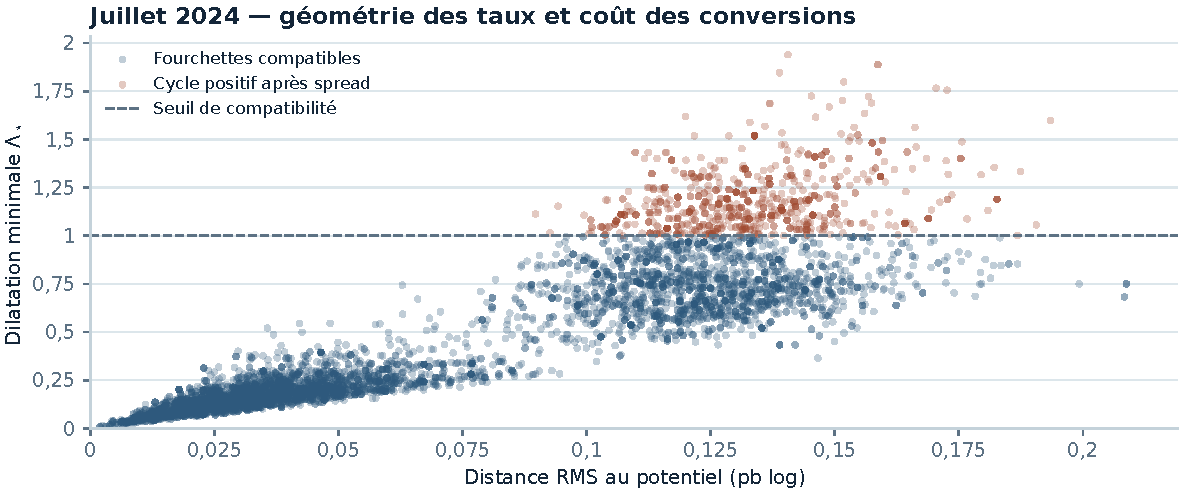
\includegraphics[width=0.99\linewidth]{geometrie_juillet.pdf}
\caption{Défaut au potentiel et dilatation minimale des demi-spreads sur les \JuilletEligibles{} instantanés frais de juillet 2024. Les points se superposent lorsque plusieurs instants portent des cotations proches ou identiques.}
\label{fig:geometrie}
\end{figure}

En juillet, la médiane de \(\sigma_H\) est de \HodgeJuilletMed{} pb log. Elle atteint \HodgeJuilletMedPositifs{} pb log parmi les signaux positifs. Parmi les \HodgeJuilletNonPositifs{} instants compatibles, \HodgeJuilletNonPositifsForts{} dépassent pourtant cette dernière valeur. Les deux groupes se recouvrent donc le long de l'axe horizontal de la figure \ref{fig:geometrie}. La taille de la courbure ne détermine pas à elle seule le signe du gain après spread.

Le facteur \(\Lambda_\star\) a une médiane de \DilatationJuilletMed{} et un maximum de \DilatationJuilletMax{}. Pour l'instant du maximum, multiplier tous les demi-spreads par ce facteur suffirait à rétablir l'existence d'un potentiel compatible. Le scénario de frais uniformes, étudié ci-après, ajoute au contraire le même nombre de points de base logarithmiques à chaque conversion.

\clearpage
\subsection{Le spread absorbe la plupart des holonomies positives}

\begin{table}[H]
\centering\small
\begin{tabular}{@{}lrrrrr@{}}
\toprule
Date & Âge $\leq 1$ s & Médian $+$ & Bid--ask $+$ & Triangle $+$ & $\mu_{\max}$\\
\midrule
10 juin & 1\,574 & 1\,574 & 0 & 0 & \ensuremath{-}0,014\\
11 juin & 2\,932 & 2\,932 & 1 & 1 & 0,002\\
12 juin & 1\,508 & 1\,508 & 0 & 0 & \ensuremath{-}0,042\\
13 juin & 2\,134 & 2\,134 & 2 & 2 & 0,182\\
14 juin & 5\,192 & 5\,192 & 8 & 8 & 0,103\\
\midrule
8 juillet & 1\,471 & 1\,471 & 1 & 1 & 0,013\\
9 juillet & 1\,412 & 1\,412 & 1 & 1 & 0,013\\
10 juillet & 1\,220 & 1\,220 & 0 & 0 & \ensuremath{-}0,031\\
11 juillet & 432 & 432 & 218 & 218 & 0,093\\
12 juillet & 2\,198 & 2\,198 & 537 & 537 & 0,090\\
\bottomrule
\end{tabular}

\caption{Comptages par jour sur la cohorte à une seconde. Les trois colonnes de signes comptent les instants avec au moins un cycle positif selon le test indiqué. $\mu_{\max}$ est la plus grande marge bid--ask de la fenêtre, en pb log par conversion.}
\label{tab:jours}
\end{table}

En juillet, \JuilletEligibles{} des \JuilletGrille{} instants, soit \JuilletEligiblesPct{}\,\%, satisfont le filtre à une seconde sur les six paires. Les taux médians donnent une holonomie positive dans au moins un sens aux \JuilletMed{} instants admissibles. Aux taux bid--ask, \JuilletNet{} instants restent positifs, soit \JuilletNetPct{}\,\%. Ils forment \JuilletEpisodes{} épisodes sur la grille et \JuilletPicDeuxJours{} de ces instants se situent les 11 et 12 juillet. Au plafond de 30 secondes, \JuilletCommunNet{} des \JuilletCommun{} instants sont positifs, soit \JuilletCommunPct{}\,\%. Modifier l'âge maximal change à la fois la composition de l'échantillon et la proportion de signaux.

Le cycle le plus favorable de juillet sur la cohorte à une seconde est EUR\,$\arrowfx$\,JPY\,$\arrowfx$\,USD\,$\arrowfx$\,EUR, le 11 juillet à \JuilletPicHeure{} UTC. La marge atteint \JuilletMarge{} pb log par conversion et \JuilletGainPic{} pb log au total. La plus ancienne des six cotations a alors \JuilletPicAge{} ms. Un coût ajouté de 0,05 pb par conversion laisse \JuilletFeeCinq{} signaux. À 0,10 pb, le nombre passe à \JuilletFeeDix{}. En juin, la marge maximale est de \JuinMarge{} pb par conversion. Le seuil constaté en juillet dépend donc de la période observée.

\begin{figure}[H]
\centering
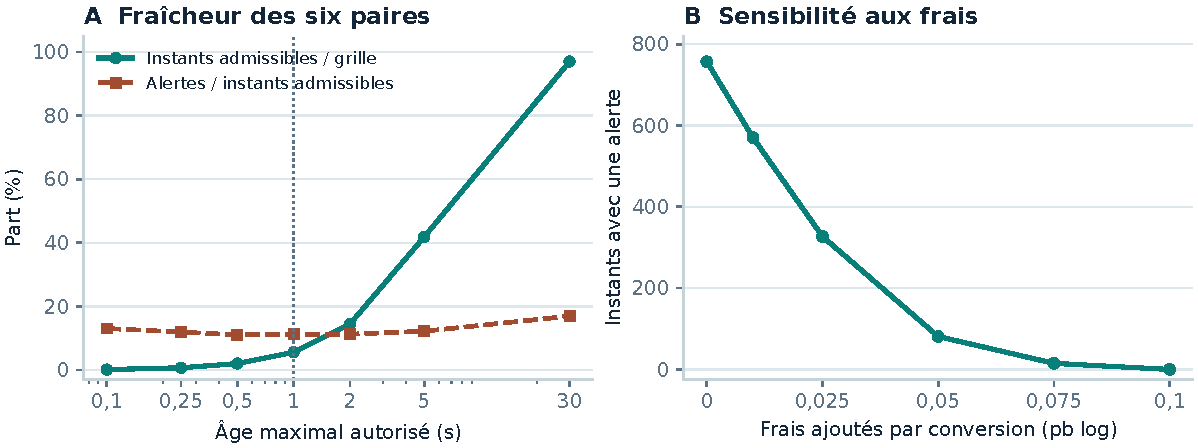
\includegraphics[width=0.99\linewidth]{fraicheur_et_frais.pdf}
\caption{Juillet. Le panneau A distingue couverture de la grille et taux de signaux parmi les instants admissibles. Le panneau B applique les frais supplémentaires à la cohorte fixe de \JuilletEligibles{} instants frais.}
\label{fig:frais}
\end{figure}

\clearpage
\subsection{Le contre-exemple théorique reste absent de la cohorte fraîche}

Un quadrilatère est positif à un seul instant frais, le 13 juin, où un triangle donne une meilleure marge par conversion. Sur les dix fenêtres, le test triangulaire retrouve ainsi tous les signaux et leur marge maximale. La section \ref{sec:contrex} donne une configuration où ce test échoue.

\begin{figure}[H]
\centering
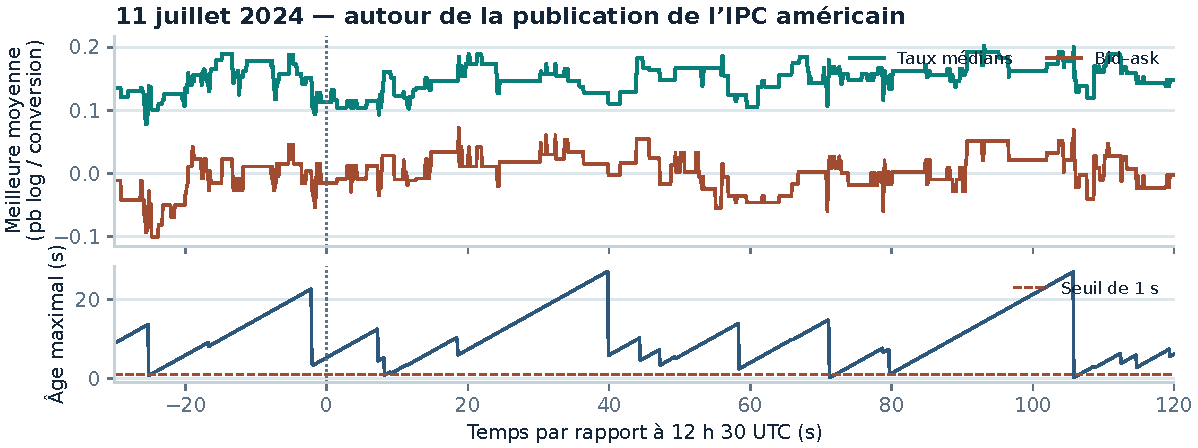
\includegraphics[width=0.99\linewidth]{ipc_juillet.pdf}
\caption{Meilleures marges et âge maximal autour de la publication du 11 juillet. Le profil utilise le plafond large de 30 secondes. L'instant zéro est l'heure de publication, et la ligne d'âge à une seconde indique le filtre de la cohorte principale.}
\label{fig:ipc}
\end{figure}

La figure \ref{fig:ipc} juxtapose la marge et l'âge de la cotation la plus ancienne. Un pic de marge peut coïncider avec des cotations de fraîcheurs différentes. L'annonce fournit ici un repère horaire.

\subsection{Un retard injecté crée des alertes en l'absence d'arbitrage}

Sur une cohorte fixe de \RetardCohorte{} instants de juillet, retarder EUR/USD de 500 ms crée \RetardReelCinqCents{} nouvelles alertes dans le flux réel et fait disparaître \RetardReelCinqCentsDisparues{} alertes de référence. Après le filtre d'âge à une seconde, \RetardReelCinqCentsFiltre{} nouvelles alertes passent encore. Dans le contrôle nul, le même retard crée \RetardNulCinqCents{} fausses alertes, dont \RetardNulCinqCentsFiltre{} après le filtre. Le filtre réduit donc l'effet sans pouvoir éliminer les erreurs d'alignement de durée inférieure à sa tolérance.

À cinq secondes, on observe \RetardNulCinqSecs{} fausses alertes dans le contrôle nul, soit \RetardNulCinqSecsPct{}\,\% de la cohorte. Le flux réel compte \RetardReelCinqSecs{} créations, les disparitions étant comptées séparément. Ce test mesure la sensibilité du diagnostic à une perturbation connue. La fréquence d'erreurs d'alignement dans l'archive reste inconnue.

\begin{figure}[H]
\centering
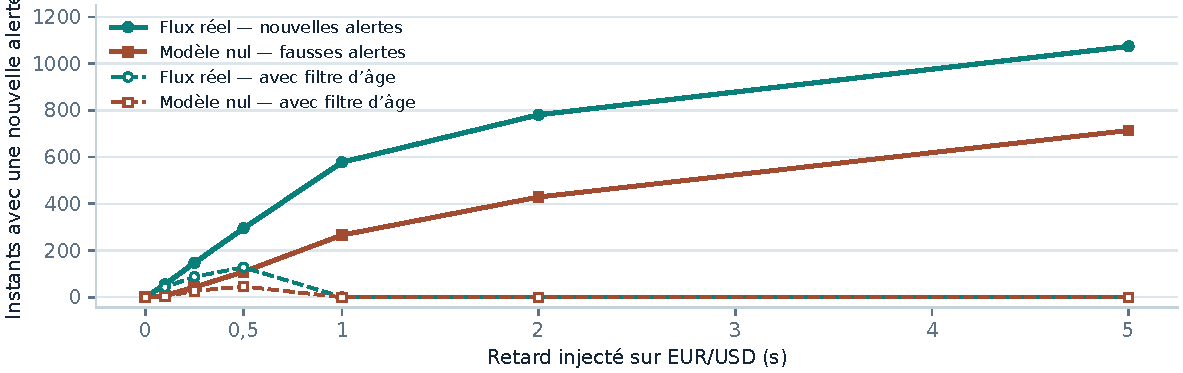
\includegraphics[width=0.99\linewidth]{retard_eurusd.pdf}
\caption{Retard ajouté à EUR/USD, sur le même ensemble d'instants à chaque abscisse. Les courbes en tirets comptent les signaux qui passent encore le filtre après injection du retard.}
\label{fig:retard}
\end{figure}

\clearpage
\subsection{Le délai réduit la part de signaux qui restent positifs}

\begin{table}[H]
\centering\small
\begin{tabular}{@{}rrrrrr@{}}
\toprule
$\Delta$ (ms) & Rejouables & Positives & Positives / rejouables & Robustes & Couverture jointe\\
\midrule
0 & 757 & 757 & 100,0\,\% & 757 & 100,0\,\%\\
100 & 608 & 512 & 84,2\,\% & 0 & 96,9\,\%\\
250 & 387 & 285 & 73,6\,\% & 0 & 97,5\,\%\\
500 & 163 & 93 & 57,1\,\% & 0 & 98,4\,\%\\
1\,000 & 69 & 42 & 60,9\,\% & 0 & 98,1\,\%\\
\bottomrule
\end{tabular}

\caption{Rejeu de juillet, après spread et avant frais ajoutés. Les deux premières colonnes de comptage se rapportent aux \JuilletNet{} alertes nominales initiales. La couverture jointe de l'enveloppe est mesurée sur les instantanés admissibles au protocole de la section \ref{sec:protocole}.}
\label{tab:latence}
\end{table}

Avec 100 ms entre les conversions, \ReplayCentOk{} des \ReplayCentEval{} signaux rejouables restent positifs. Cela représente \ReplayCentPartInitiale{}\,\% des \JuilletNet{} alertes initiales. À 500 ms, \ReplayCinqCentsOk{} des \ReplayCinqCentsEval{} signaux rejouables restent positifs, soit \ReplayCinqCentsPartInitiale{}\,\% des alertes initiales. La part positive conditionnelle au rejeu peut remonter lorsqu'une grande partie de l'échantillon devient non rejouable. La comparaison sur la cohorte initiale permet de voir cette attrition.

Un filtre initial plus strict, à 250 ms sur les six paires, ne conserve que \ReplayCentStrictTotal{} alertes. À 100 ms de délai par conversion, elles sont toutes rejouables et \ReplayCentStrictOk{} restent positives. Ce filtre réduit le nombre de cas non rejouables, avec un compromis sur la quantité de signaux retenus.

\begin{figure}[H]
\centering
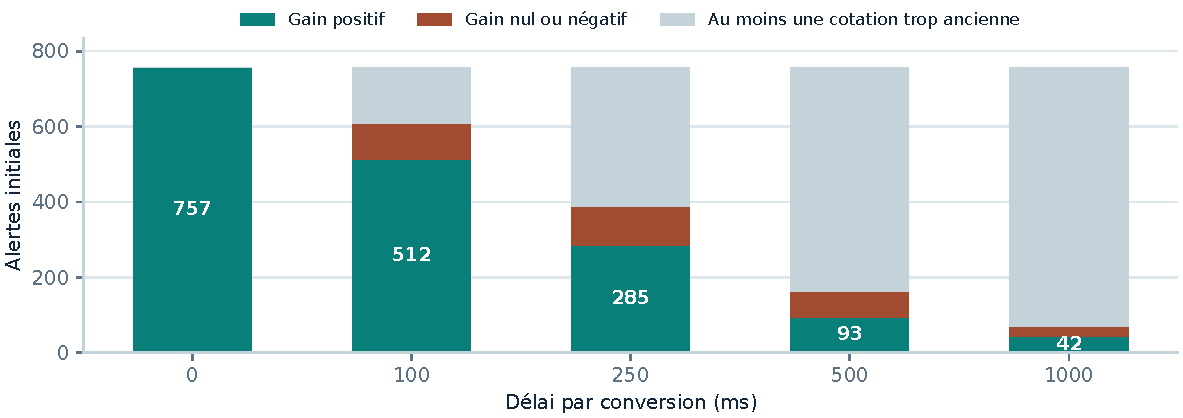
\includegraphics[width=0.99\linewidth]{rejeu.pdf}
\caption{Décomposition des \JuilletNet{} alertes nominales de juillet au fil du délai de conversion. La zone grise correspond à une étape dont la cotation est trop ancienne au moment du rejeu.}
\label{fig:rejeu}
\end{figure}

\subsection{L'enveloppe empirique est trop large pour trancher}

À 100 ms, les rayons directionnels appris en juin vont de \RayonCentMin{} à \RayonCentMax{} pb log par arête. Même le plus petit rayon excède la meilleure moyenne nominale de juillet, \JuilletMarge{} pb par conversion. Ainsi, pour tout cycle de juillet, la moyenne inférieure est négative. Pour chaque délai strictement positif testé, la règle robuste classe tous les instants frais comme indéterminés dans cette expérience, avec zéro acceptation et zéro rejet par borne supérieure. La couverture jointe à 100 ms atteint \ReplayCentPairesOk{}\,\% sur les instantanés éligibles et \ReplayCentAlertesCouv{}\,\% sur les alertes initiales éligibles. Ces mesures donnent le compromis observé entre couverture des chocs et capacité à conclure. La boîte additionne des variations défavorables sur les arêtes. Une partie des variations communes peut se compenser sur un cycle.

\clearpage
\clearpage
\part{Expérience 1}
\section{Holonomie globale sur un cylindre de conversions}
\label{sec:experience-un}

\subsection{Question et marché contrôlé}

Peut-on avoir une courbure locale nulle, une période globale non nulle et un gain après coûts ? Pour isoler ce mécanisme, on construit un réseau de huit sommets, douze arêtes non orientées et quatre faces carrées. Les sommets peuvent se lire comme quatre devises présentes sur deux plateformes. Les liens horizontaux autorisent les conversions sur chaque anneau, les liens verticaux les transferts entre plateformes. Les autres conversions sont absentes du modèle.

\begin{center}
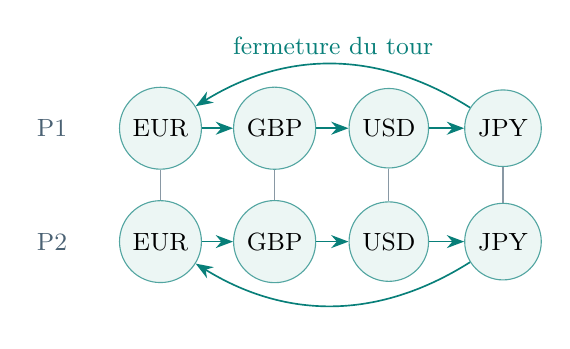
\begin{tikzpicture}[x=1.45cm,y=0.8cm,
  currency/.style={circle,draw=teal!70,fill=pale,minimum size=8mm,font=\small},
  conv/.style={-{Stealth[length=2.2mm]},semithick,teal}]
 \foreach \name/\x/\text in {a/0/EUR,b/1/GBP,c/2/USD,d/3/JPY}{
   \node[currency] (\name) at (\x,0.9) {\text};
   \node[currency] (\name2) at (\x,-0.9) {\text};
   \draw[muted!65] (\name) -- (\name2);
 }
 \draw[conv] (a)--(b); \draw[conv] (b)--(c); \draw[conv] (c)--(d);
 \draw[conv] (a2)--(b2); \draw[conv] (b2)--(c2); \draw[conv] (c2)--(d2);
 \draw[conv] (d) to[bend right=32] node[above,font=\small] {fermeture du tour} (a);
 \draw[conv] (d2) to[bend left=32] (a2);
 \node[font=\small,text=muted] at (-0.95,0.9) {P1};
 \node[font=\small,text=muted] at (-0.95,-0.9) {P2};
\end{tikzpicture}
\end{center}

Les quatre faces sont les rectangles entre les deux anneaux, y compris celui qui ferme le tour. Cette identification donne un cylindre cellulaire. Les faces sont fixées par la construction du réseau. Le graphe de cotations complet à quatre devises de l'étude HistData a une autre topologie.

Dans une orientation suivant chaque tour, la cochaîne \(\eta_0\) vaut \(1/4\) sur les huit liens horizontaux et zéro sur les quatre liens verticaux. On impose
\[
 m=D_0h+\alpha\eta_0,\qquad
 D_1\eta_0=0,\quad D_0^{\mathsf T}\eta_0=0 .
\]
Le potentiel \(h\) est tiré une fois à graine fixée et sert de changement d'unités local. Dans la jauge \(h=0\), les liens de transfert ont un milieu égal à un. La période \(\alpha\), exprimée en pb logarithmiques, règle le défaut global. Le calcul donne \(\operatorname{rang}D_0=7\), \(\operatorname{rang}D_1=4\) et
\(\dim H^1=12-7-4=1\). La composante harmonique est donc entièrement paramétrée par \(\alpha\).

Chaque direction d'une arête paie le même demi-spread \(s\ge0\). Les taux du modèle sont \(r_{ij}=\exp[(m_{ij}-s)/10^4]\), et le taux inverse exécutable est \(\exp[(-m_{ij}-s)/10^4]\). La fourchette est ordonnée. La période du tour \(C\) dans l'orientation choisie vaut \(\alpha\). Le sens favorable paie quatre coûts, d'où
\begin{equation}
 \log H(C)=\frac{\alpha}{10^4},\qquad
 G_{\mathrm{tour}}=|\alpha|-4s
 \quad\text{en pb logarithmiques}.
 \label{eq:experience-un-seuil}
\end{equation}
Sur un cycle, le gradient \(D_0h\) s'annule. Chaque arête harmonique contribue au plus \(|\alpha|/4\) et chaque arête paie \(s\). Un tour atteint cette moyenne maximale, donc un cycle positif existe exactement lorsque \(|\alpha|>4s\).

\clearpage
\subsection{Résultats et lecture géométrique}

On énumère les \ExpUnCycles{} cycles dirigés simples du réseau. La grille de \ExpUnGrille{} scénarios combine \(161\) valeurs de \(\alpha\) entre \(-2\) et \(2\) pb et \(121\) valeurs de \(s\) entre \(0\) et \(0{,}6\) pb. Le signe calculé coïncide avec \eqref{eq:experience-un-seuil} sur chaque scénario, avec la tolérance numérique du rapport. On compte \ExpUnPositifs{} scénarios avec un gain strictement positif.

\begin{figure}[H]
\centering
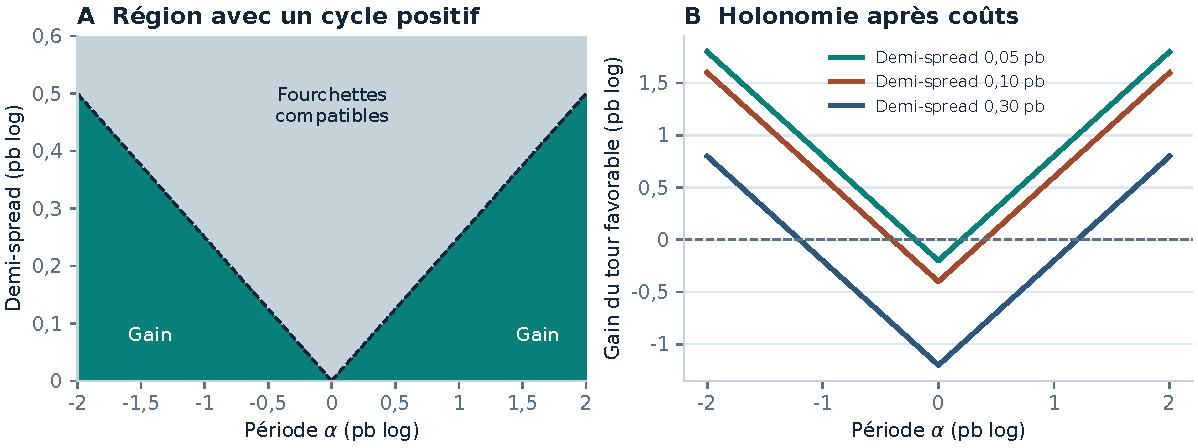
\includegraphics[width=0.99\linewidth]{experience_un_phase.pdf}
\caption{Expérience 1. La zone verte admet un cycle positif. Les lignes en tirets sont les frontières \(|\alpha|=4s\). À droite, le gain du tour favorable est tracé pour trois niveaux de coût.}
\label{fig:experience-un}
\end{figure}

\begin{table}[H]
\centering\small
\begin{tabular}{@{}rrrrr@{}}
\toprule
\(\alpha\) & \(s\) & Coût du tour & Gain du tour favorable & \(\Lambda_\star\)\\
\midrule
0 & 0,1 & 0,4 & \(-0,4\) & 0\\
0,3 & 0,1 & 0,4 & \(-0,1\) & 0,75\\
1 & 0,1 & 0,4 & 0,6 & 2,50\\
1 & 0,3 & 1,2 & \(-0,2\) & 0,83\\
\bottomrule
\end{tabular}
\caption{Cas contrôlés. Les quatre premières colonnes sont en pb logarithmiques. La dilatation \(\Lambda_\star=|\alpha|/(4s)\) est sans dimension.}
\end{table}

La circulation autour de chaque face reste inférieure à \(3\times10^{-14}\) pb en valeur absolue sur la grille. Un changement aléatoire de jauge modifie les périodes d'au plus \ExpUnJauge{} pb. La projection sur \(\eta_0\) retrouve \(\alpha\) à moins de \(4\times10^{-14}\) pb près. Ces écarts sont ceux de l'arithmétique flottante.

Les deux lignes à \(\alpha=1\) montrent que la même holonomie globale peut accompagner des signes de gain opposés selon les coûts. La ligne à \(\alpha=0{,}3\) montre une période non nulle absorbée par le spread. Dans les scénarios profitables, un test qui ne lirait que les quatre flux de faces donnerait toujours zéro. Le calcul des périodes ou la recherche globale des cycles détecte le tour favorable.

L'expérience réalise numériquement la distinction entre platitude et exactitude de la première partie. Le seuil financier est déduit de cette période et du budget de spread. Ce résultat est établi analytiquement avant le calcul. Les données HistData servent ensuite à une autre question, celle de la robustesse temporelle des signaux.

\clearpage
\part{Expérience 2}
\section{Certifier directement les circulations sur HistData}
\label{sec:experience-deux}

\subsection{Des erreurs d'arêtes aux erreurs de chemins}

L'enveloppe de la section \ref{sec:marge} traite les variations de chaque arête séparément. Une même variation peut se compenser avec d'autres le long d'un cycle. On conserve les six paires, les dix fenêtres et les délais \(\Delta\in\{0,100,250,500,1000\}\) ms du protocole initial. Les cinq fenêtres de juin calibrent les seuils. Celles de juillet évaluent les règles figées.

Pour un cycle \(C\) de longueur \(\ell_C\), la notation \(g_C(t)=G_C(t)/\ell_C\) désigne son log-gain nominal moyen par conversion. Le rejeu au délai \(\Delta\), avec le point de départ canonique déjà fixé, donne \(g_C^\Delta(t)\). L'erreur est
\[
 e_C(t,\Delta)=g_C^\Delta(t)-g_C(t).
\]
Ces quantités sont des rapports de transports relativement à la détention dans la devise de départ, selon la convention de la section \ref{sec:temps}. Dans les unités de cotation du calcul, le portage vaut zéro. Cette convention permet de calculer les erreurs à partir des cotations archivées.

On compare trois méthodes, aux quantiles \(q=90\,\%,95\,\%,99\,\%\), tous déclarés comme niveaux de sensibilité.
\begin{enumerate}
 \item \textbf{Arêtes marginales.} La méthode initiale calcule un quantile \(u_e\) sur chaque arête. Son rayon moyen pour le cycle est \(u_C=\sum_{e\in C}u_e/\ell_C\).
 \item \textbf{Arêtes simultanées.} On calibre un rayon commun \(u_A=\widehat Q_q(\max_{e,1\le k\le4}|a_e(t+k\Delta)-a_e(t)|)\). Il borne chaque moyenne de cycle sous le même événement.
 \item \textbf{Cycles simultanés.} On calibre directement
 \begin{equation}
  u_H(\Delta)=\widehat Q_q\!\left(\max_{C\in\mathcal C}|e_C(t,\Delta)|\right).
  \label{eq:cycle-envelope}
 \end{equation}
\end{enumerate}
Le maximum de \eqref{eq:cycle-envelope} couvre les vingt cycles avant le choix d'un témoin. Le quantile prend l'observation d'ordre supérieur. Les \(13\,340\) instants frais de juin sont tous admissibles au contrôle large des cotations futures, pour chacun des délais.

\begin{proposition}[Borne directe par circulation]
Si \(|e_C|\le u_C\) pour tous les cycles, alors \(g_C^\Delta\ge g_C-u_C\). Un cycle choisi en maximisant \(g_C-u_C\) et dont la borne est positive reste positif au rejeu. Si \(\max_C(g_C+u_C)\le0\), tous les cycles du protocole ont un gain non positif. De plus, pour les deux contrôles simultanés ci-dessus, \(u_H\le u_A\) sur la calibration.
\end{proposition}
\begin{proof}
Les deux décisions découlent des bornes sur \(e_C\). Pour le dernier point, une erreur moyenne de cycle est une moyenne d'erreurs d'arêtes à leurs rangs de conversion respectifs. Son module est au plus le maximum des erreurs d'arêtes sur tous les rangs. L'inégalité se conserve pour le maximum sur les cycles et pour le quantile empirique.
\end{proof}

\clearpage
\subsection{Résultats au quantile de 99 \%}

Les couvertures sont mesurées sur le même ensemble d'instants dont les quatre graphes futurs sont admissibles au plafond de 30 secondes. Le rejeu d'un témoin exige toujours un âge d'au plus une seconde pour chaque cotation utilisée. La couverture des cycles mesure l'événement conjoint \(|e_C|\le u_C\) pour les vingt cycles. Pour les méthodes d'arêtes, on mesure aussi leur événement conjoint sur les douze directions et quatre rangs.

\begin{table}[H]
\centering\small
\begin{tabular}{@{}lrrrr@{}}
\toprule
Méthode & Rayon & Couv. des cycles & Acceptés & Rejetés\\
\midrule
Arêtes marginales & 0,356--0,535 & 100,00\,\% & 0 & 0\\
Arêtes simultanées & 0,701 & 100,00\,\% & 0 & 0\\
Cycles simultanés & 0,237 & 99,42\,\% & 0 & 0\\
\bottomrule
\end{tabular}

\caption{Expérience 2, juillet, délai de 100 ms, quantile de calibration de 99 \%. Les rayons sont en pb log par conversion. Les comptages portent sur \(6\,733\) instantanés frais.}
\label{tab:experience-deux}
\end{table}

À 100 ms, le rayon direct est de \(0{,}2365\) pb par conversion, contre \(0{,}7009\) pour le contrôle simultané des arêtes. Il est donc environ \(2{,}96\) fois plus petit. Pour la boîte marginale initiale, les rayons moyens des cycles vont de \(0{,}3564\) à \(0{,}5354\) pb. Le gain nominal maximal de juillet est de \(0{,}0930\) pb par conversion. Même l'enveloppe directe absorbe donc toute la meilleure marge nominale.

\begin{figure}[H]
\centering
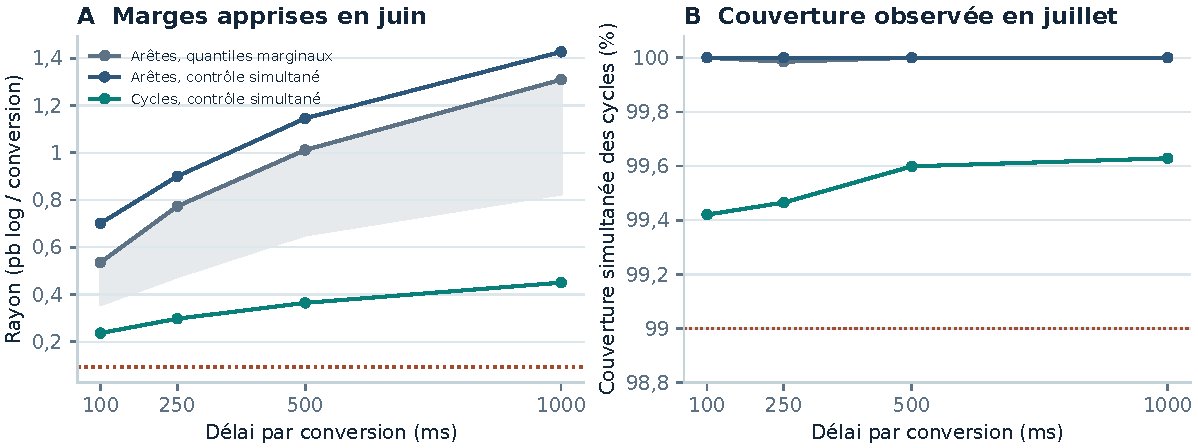
\includegraphics[width=0.99\linewidth]{experience_deux_certificats.pdf}
\caption{Expérience 2. À gauche, les rayons appris au quantile de 99 \%. La zone grise est l'intervalle des rayons moyens des cycles pour la boîte marginale. La ligne pointillée rouge est la meilleure marge nominale de juillet. À droite, couverture simultanée des erreurs des cycles au test.}
\label{fig:experience-deux}
\end{figure}

Pour chaque délai strictement positif testé et les trois quantiles, aucune méthode n'accepte de cycle robuste. Au quantile de 99 \%, les trois méthodes laissent aussi tous les cas indéterminés. La borne par cycle resserre les intervalles sans produire de gain certifié dans ces fenêtres.

À 100 ms, l'événement conjoint sur les arêtes de la boîte marginale couvre \(96{,}87\,\%\) des instantanés, tandis que les bornes qu'elle induit sur les cycles couvrent \(100\,\%\). La compensation des erreurs explique cette différence. Pour le rayon direct par cycle, la couverture est de \(99{,}42\,\%\), contre \(99{,}47\,\%\), \(99{,}60\,\%\) et \(99{,}63\,\%\) aux trois délais suivants. Les probabilités de test sont observées sur juillet, après calibration sur juin.

\clearpage
\subsection{La possibilité de rejeter dépend de la couverture choisie}

Au délai de 100 ms, le passage de 99 \% à 90 \% réduit le rayon direct de \(0{,}237\) à \(0{,}119\) pb par conversion. Cela permet de rejeter certains graphes nominaux par borne supérieure.

\begin{table}[H]
\centering\small
\begin{tabular}{@{}rrrrr@{}}
\toprule
Quantile & Rayon & Couv. & Rejetés & Rejets contredits\\
\midrule
90\,\% & 0,119 & 91,83\,\% & 894 & 3\\
95\,\% & 0,159 & 96,57\,\% & 5 & 0\\
99\,\% & 0,237 & 99,42\,\% & 0 & 0\\
\bottomrule
\end{tabular}

\caption{Sensibilité de la règle par cycles, juillet et délai de 100 ms. Un rejet contredit est un instant où un cycle aux étapes rejouables à une seconde donne ensuite un gain positif.}
\label{tab:experience-deux-sensibilite}
\end{table}

Au quantile de 90 \%, les \(894\) rejets représentent \(13{,}28\,\%\) de la cohorte fraîche. Trois d'entre eux sont contredits par un cycle positif rejouable. Chacun de ces trois cas se situe hors de l'enveloppe calibrée. La couverture jointe des cycles est de \(91{,}83\,\%\). Au quantile de 95 \%, on obtient cinq rejets et aucun rejet contredit dans ce test. Au quantile de 99 \%, aucun rejet n'est prononcé. Les acceptations robustes restent nulles dans les trois cas.

Le rayon direct conserve les compensations que les contraintes séparées sur les arêtes peuvent perdre. Il apporte ici un résultat mesurable sur la largeur des intervalles et sur les décisions de rejet à plus faible quantile. L'expérience ne met en évidence aucune acceptation robuste profitable à délai positif.

La preuve du certificat est déterministe sous la borne annoncée. Le quantile de calibration donne une règle empirique. Les observations voisines partagent des ticks et les deux périodes ont des comportements différents. On rapporte donc les fréquences par date dans \filepath{results/exp2_resultats.csv}, ainsi que les couvertures globales et celles des alertes initiales. Ces cinq fenêtres de test décrivent une expérience chronologique sur ce flux.

\begin{callout}{Reproduction de l'expérience sur les prix archivés}
Le cache \filepath{data/exp2_cycle_panels.npz} conserve les gains nominaux et rejoués, les erreurs maximales d'arêtes et les masques de fraîcheur. Il permet de recalculer les quantiles et les décisions. La commande de reconstruction depuis les douze archives vérifie leurs empreintes avant toute extraction. Le cache stocke des observables de cycles, avec les diagnostics d'erreurs nécessaires aux comparateurs.
\end{callout}

\clearpage
\part{Expérience 3}
\section{Retards, transport temporel et fausses alertes}
\label{sec:experience-trois}

\subsection{Un modèle de référence sans arbitrage dynamique}

On travaille sous une mesure de probabilité \(Q\), avec l'USD comme numéraire constant et des taux d'intérêt nuls. Pour les trois autres devises, les valeurs en USD sont
\begin{equation}
 V_i(t)=\exp\!\left(\frac{\sigma_i}{10^4}W_i(t)
                     -\frac12\left(\frac{\sigma_i}{10^4}\right)^2t\right),
 \qquad m_{ij}(t)=10^4\log\frac{V_i(t)}{V_j(t)} .
 \label{eq:exp3-martingale}
\end{equation}
Les \(V_i\) sont des martingales exponentielles positives à volatilités constantes sous \(Q\). Ce modèle fournit donc un marché de référence frictionless sans arbitrage sous les hypothèses usuelles des stratégies admissibles. Ajouter les spreads restreint les possibilités de transaction \cite{delbaen}. À chaque instant, les milieux sont exacts et toute moyenne de cycle synchrone paie le demi-spread de \(0{,}1\) pb par conversion.

Les volatilités de EUR, GBP et JPY sont \(0{,}45\), \(0{,}55\) et \(0{,}60\) pb par racine de seconde. Les bruits s'écrivent \(W_i=0{,}6B_0+0{,}8B_i\), avec des browniens \(B\) indépendants. Ces paramètres définissent un marché simulé pédagogique. Ils sont fixés avant les calculs et ne sont pas ajustés au flux HistData.

On simule \ExpTroisRepliques{} trajectoires indépendantes, de graines \(110603\) à \(110642\), à pas de 10 ms. Sur chacune, \(1\,100\) décisions sont prises de 5 s à 114,9 s à pas de 100 ms. Les trajectoires couvrent aussi les conversions futures. Les données sont générées directement aux instants de grille par les incréments gaussiens exacts de \eqref{eq:exp3-martingale}.

\subsection{Observation asynchrone et exécution}

Les paires sont mises à jour indépendamment. Pour un paramètre d'intensité \(\tau\), la probabilité de mise à jour à un pas de 10 ms est \(1-e^{-10/\tau}\). On teste \(\tau=20,100,500\) ms. Sur la grille, l'attente moyenne effective vaut \(10/(1-e^{-10/\tau})\), soit \(25{,}4\), \(105{,}1\) et \(505{,}0\) ms. Les figures indiquent \(\tau\). Un second paramètre retarde seulement la source EUR/USD de \(0,100,500,1000\) ms. Un scénario supplémentaire suspend les mises à jour d'EUR/GBP entre 40 et 45 s. Deux contrôles utilisent des mises à jour synchrones, avec zéro ou 500 ms de retard sur EUR/USD. On obtient quinze scénarios par trajectoire.

À chaque décision, le détecteur choisit le cycle de meilleure moyenne sur les dernières cotations observées. La vérité synchrone au même instant est connue et chaque cycle y est déficitaire. Les signaux positifs de la matrice décalée sont donc de fausses alertes instantanées relativement à cette vérité.

Pour mesurer ce qui se passe ensuite, on exécute le cycle choisi aux \emph{prix courants du modèle} à \(t+k\Delta\), pour \(\Delta=0,100,500,1000\) ms. Le sens, la rotation et les devises sont fixés à la décision. Les gains futurs sont des résultats de transactions exposées à l'évolution des prix. Les cotations archivées dans la matrice décalée servent à la décision, tandis que les conversions utilisent les prix du marché simulé au moment de l'ordre.

\clearpage
\subsection{Les retards produisent des alertes même avec des ticks récents}

\begin{figure}[H]
\centering
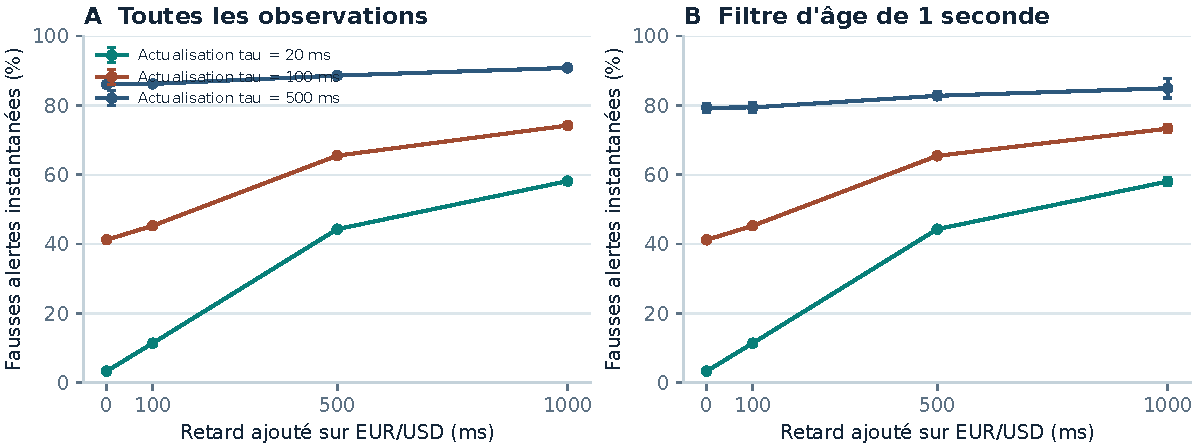
\includegraphics[width=0.99\linewidth]{experience_trois_retards.pdf}
\caption{Expérience 3. Fréquence moyenne des fausses alertes sur quarante trajectoires. Les barres indiquent la moyenne \(\pm1{,}96\) fois son erreur standard entre trajectoires indépendantes. Le panneau B conditionne aux cotations âgées d'au plus une seconde.}
\label{fig:experience-trois-retard}
\end{figure}

Sans retard et avec des mises à jour synchrones, on compte zéro alerte. Retarder uniquement EUR/USD de 500 ms, en gardant les autres paires synchrones, donne une fréquence moyenne de \(34{,}94\,\%\). Avec une échelle d'actualisation de 20 ms et aucun retard ajouté, cette fréquence est de \(3{,}35\,\%\). Avec une échelle d'actualisation de 100 ms et un retard ajouté de 500 ms, elle atteint \(65{,}51\,\%\) sur toutes les décisions et \(65{,}45\,\%\) après le filtre d'âge à une seconde.

La panne d'EUR/GBP augmente la fréquence globale à \(66{,}66\,\%\) dans ce dernier scénario. Une fois le filtre d'âge appliqué, elle est de \(65{,}60\,\%\). Ces valeurs caractérisent le marché simulé aux volatilités et au spread choisis. Elles quantifient le mécanisme de décalage sans estimer sa fréquence sur un marché réel.

\begin{figure}[H]
\centering
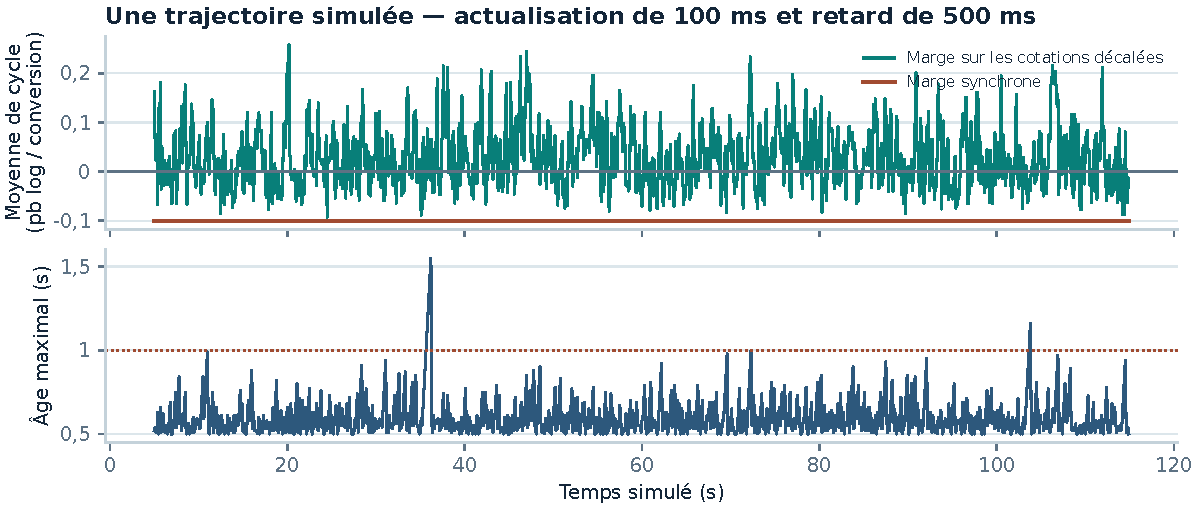
\includegraphics[width=0.99\linewidth]{experience_trois_trajectoire.pdf}
\caption{Une trajectoire du scénario avec une échelle d'actualisation de 100 ms et retard EUR/USD de 500 ms. La marge reconstruite oscille et devient positive. La marge synchrone reste à \(-0{,}1\) pb par conversion. Les âges restent souvent sous le filtre d'une seconde.}
\label{fig:experience-trois-trace}
\end{figure}

\clearpage
\subsection{Un gain futur positif peut accompagner une moyenne négative}

On retient le scénario avec une échelle d'actualisation de 100 ms et retard EUR/USD de 500 ms. Les \(28\,595\) alertes initiales passant le filtre de fraîcheur forment une cohorte commune aux quatre délais d'exécution.

\begin{table}[H]
\centering\small
\begin{tabular}{@{}rrrr@{}}
\toprule
Délai (ms) & Rejeux positifs & Part positive & Gain moyen\\
\midrule
0 & 0 & 0,00\,\% & \ensuremath{-}0,1000\\
100 & 3\,033 & 10,61\,\% & \ensuremath{-}0,1002\\
500 & 8\,207 & 28,70\,\% & \ensuremath{-}0,1003\\
1000 & 9\,883 & 34,56\,\% & \ensuremath{-}0,1006\\
\bottomrule
\end{tabular}

\caption{Rejeu des \(28\,595\) alertes simulées fraîches, réparties sur quarante trajectoires. Le gain est en pb log par conversion. La moyenne de la dernière colonne donne un poids égal à chaque trajectoire.}
\label{tab:experience-trois-rejeu}
\end{table}

\begin{figure}[H]
\centering
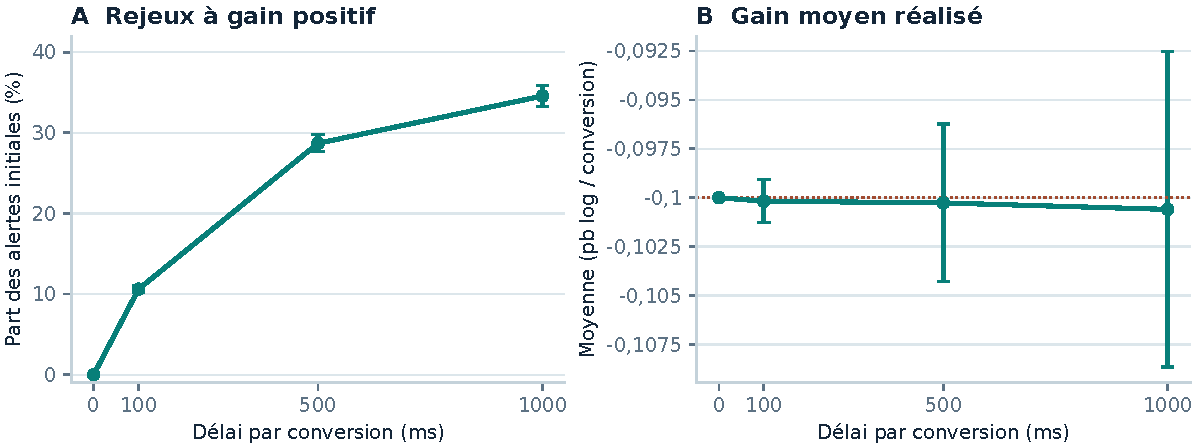
\includegraphics[width=0.99\linewidth]{experience_trois_rejeu.pdf}
\caption{Expérience 3, même scénario. La fréquence positive augmente avec le délai, tandis que le gain moyen reste voisin de \(-0{,}1\) pb par conversion. Les intervalles sont calculés entre trajectoires indépendantes.}
\label{fig:experience-trois-rejeu}
\end{figure}

À délai nul, aucune de ces alertes ne donne de gain aux vrais taux synchrones. À une seconde par conversion, \(9\,883\) rejeux sont positifs, soit \(34{,}56\,\%\), avec un gain moyen de \(-0{,}1006\) pb par conversion. L'allongement du délai ajoute une exposition aux variations du marché. Un signe positif réalisé sur certaines trajectoires accompagne ici une moyenne négative et le risque de perdre.

\subsection{Vérification de jauge sur les chemins temporels}

On applique une transformation dépendante du temps \(\chi_i(t)=3\sin(t/7+i)+11i\), en coordonnées logarithmiques de calcul. La conversion \(i\to j\) à \(t_k\) reçoit l'incrément \(\chi_j(t_k)-\chi_i(t_k)\). La détention en \(i\) entre deux étapes reçoit \(\chi_i(t_k)-\chi_i(t_{k-1})\). La référence détenue dans la devise initiale reçoit \(\chi_{i_0}(T)-\chi_{i_0}(t)\).

La somme des incréments le long du trajet télescope en ce dernier terme. En soustrayant la détention de référence, le gain est invariant. Le contrôle est effectué sur chaque chemin rejoué dans les quinze scénarios, les quatre délais et les quarante trajectoires. L'écart maximal vaut \ExpTroisErreurJauge{} pb logarithmiques au total. L'expérience met ainsi en œuvre le fibré sur les sommets \((i,t)\) et sa connexion temporelle.



\clearpage
\section{Conclusion}
\label{sec:conclusion}

Sur une variété, l'annulation de la courbure rend les périodes homotopiquement invariantes. Leur annulation rend la connexion exacte. Sur le complexe complet des quatre devises, les triangles engendrent les cycles et suffisent à tester l'exactitude des milieux. Le bid--ask transforme cette égalité en un problème de faisabilité dans les fourchettes. Le quadrilatère construit à la section \ref{sec:contrex} montre qu'alors un test triangulaire peut manquer un gain. Sur la cohorte étudiée, il coïncide avec le test global de signe.

L'évaluation empirique sépare l'écart géométrique au potentiel, le budget de spread et la stabilité temporelle. Les défauts de potentiel observés se recouvrent entre signaux positifs et fourchettes compatibles. Un coût additionnel de 0,10 pb par conversion efface tous les signaux frais de juillet. Le contrôle nul et le rejeu montrent la sensibilité à l'alignement temporel. Dans cette calibration, le certificat par boîte classe les cas à délai positif comme indéterminés.

Les trois expériences apportent des contrôles complémentaires. Sur le cylindre, la période harmonique fait apparaître le seuil exact \(|\alpha|>4s\), même lorsque tous les flux de faces sont nuls. Sur HistData, l'enveloppe directe des cycles réduit les rayons, avec une couverture mesurée hors période, mais les délais positifs restent sans acceptation robuste. Dans le modèle martingale, les cotations retardées créent des alertes qui disparaissent aux prix synchrones. Les gains séquentiels deviennent aléatoires lorsque le délai augmente, et la transformation des liens de détention préserve l'invariance de jauge.

L'interprétation financière est circonscrite à ce flux, ces fenêtres et ces règles de reconstruction. L'archive documente des prix affichés. Une étude de gains exécutés demanderait aussi des tailles disponibles, des journaux d'ordres et des conditions de frais, de financement et de règlement. Les observations voisines partagent souvent les mêmes ticks. Les proportions sont donc descriptives et l'extension à d'autres régimes de marché demanderait des périodes et des sources supplémentaires.

\begin{callout}{Fil conducteur pour la présentation}
Comparer le cylindre, où un tour garde une holonomie malgré \(F=0\), au graphe complet, où les faces contrôlent toutes les circulations. Introduire ensuite le bid--ask et le quadrilatère. La figure \ref{fig:geometrie} illustre sur des données de marché la différence entre la courbure des milieux et la compatibilité des fourchettes.
\end{callout}

\clearpage
\begin{thebibliography}{99}
\small
\setlength{\itemsep}{3pt}
\phantomsection\label{sec:references}\addcontentsline{toc}{section}{Références}
\bibitem{tong}
D. Tong. \emph{Gauge Theory}, chapitres 1 et 4.
Notes de cours, University of Cambridge.
\href{https://www.damtp.cam.ac.uk/user/tong/gaugetheory.html}{Notes de cours}.

\bibitem{nakahara}
M. Nakahara. \emph{Geometry, Topology and Physics}, 2\textsuperscript{e} éd.,
Institute of Physics Publishing, 2003.
\href{https://www.routledge.com/Geometry-Topology-and-Physics-2nd-Edition/Nakahara/p/book/9780750306065}{Notice de l'éditeur}.

\bibitem{botttu}
R. Bott et L. W. Tu. \emph{Differential Forms in Algebraic Topology}.
Springer, 1982.
\href{https://doi.org/10.1007/978-1-4757-3951-0}{Ouvrage}.

\bibitem{hodge}
X. Jiang, L.-H. Lim, Y. Yao et Y. Ye. \emph{Statistical ranking and combinatorial Hodge theory}.
Mathematical Programming, 127, 203--244, 2011.
\href{https://doi.org/10.1007/s10107-010-0419-x}{Article}.

\bibitem{ilinski97}
K. Ilinski. \emph{Physics of Finance}. 1997.
\href{https://arxiv.org/abs/hep-th/9710148}{arXiv:hep-th/9710148}.

\bibitem{ilinski}
K. Ilinski. \emph{Gauge geometry of financial markets}.
Journal of Physics A: Mathematical and General, 33, L5, 2000.
\href{https://doi.org/10.1088/0305-4470/33/1/102}{DOI 10.1088/0305-4470/33/1/102}.

\bibitem{sornette}
D. Sornette. \emph{Gauge theory of Finance?} 1998.
\href{https://arxiv.org/abs/cond-mat/9804045}{arXiv:cond-mat/9804045}.

\bibitem{vazquez}
S. E. Vazquez et S. Farinelli. \emph{Gauge invariance, geometry and arbitrage}.
Journal of Investment Strategies, 1(2), 23--66, 2012.
\href{https://arxiv.org/abs/0908.3043}{Version arXiv:0908.3043}.

\bibitem{farinelli}
S. Farinelli et H. Takada. \emph{The Black--Scholes equation in the presence of arbitrage}.
Quantitative Finance, 22(12), 2155--2170, 2022.
\href{https://doi.org/10.1080/14697688.2022.2117075}{DOI 10.1080/14697688.2022.2117075}.

\bibitem{sedgewick}
R. Sedgewick et K. Wayne. \emph{Algorithms}, 4\textsuperscript{e} éd., section 4.4,
Addison--Wesley, 2011.
\href{https://algs4.cs.princeton.edu/44sp/Arbitrage.java.html}{Exemple de détection d'arbitrage}.

\bibitem{karp}
R. M. Karp. \emph{A characterization of the minimum cycle mean in a digraph}.
Discrete Mathematics, 23(3), 309--311, 1978.
\href{https://doi.org/10.1016/0012-365X(78)90011-0}{DOI 10.1016/0012-365X(78)90011-0}.

\bibitem{delbaen}
F. Delbaen et W. Schachermayer. \emph{A general version of the fundamental theorem of asset pricing}.
Mathematische Annalen, 300, 463--520, 1994.
\href{https://eudml.org/doc/165264}{Notice et texte}.

\bibitem{schachermayer}
W. Schachermayer. \emph{The fundamental theorem of asset pricing under proportional transaction costs in finite discrete time}.
Mathematical Finance, 14(1), 19--48, 2004.
\href{https://doi.org/10.1111/j.0960-1627.2004.00180.x}{DOI 10.1111/j.0960-1627.2004.00180.x}.

\bibitem{geman}
H. Geman, N. El Karoui et J.-C. Rochet. \emph{Changes of numéraire, changes of probability measure and option pricing}.
Journal of Applied Probability, 32(2), 443--458, 1995.
\href{https://doi.org/10.2307/3215299}{DOI 10.2307/3215299}.

\bibitem{aiba}
Y. Aiba, N. Hatano, H. Takayasu, K. Marumo et T. Shimizu.
\emph{Triangular arbitrage as an interaction among foreign exchange rates}.
Physica A, 310(3--4), 467--479, 2002.
\href{https://doi.org/10.1016/S0378-4371(02)00799-9}{DOI 10.1016/S0378-4371(02)00799-9}.

\bibitem{fenn}
D. J. Fenn, S. D. Howison, M. McDonald, S. Williams et N. F. Johnson.
\emph{The mirage of triangular arbitrage in the spot foreign exchange market}.
International Journal of Theoretical and Applied Finance, 12(8), 1105--1123, 2009.
\href{https://doi.org/10.1142/S0219024909005609}{DOI 10.1142/S0219024909005609}.

\bibitem{ito}
T. Ito, K. Yamada, M. Takayasu et H. Takayasu.
\emph{Execution risk and arbitrage opportunities in the foreign exchange markets}.
NBER Working Paper 26706, 2020.
\href{https://doi.org/10.3386/w26706}{DOI 10.3386/w26706}.

\bibitem{cross}
R. Cross, V. Kozyakin, B. O'Callaghan, A. Pokrovskii et A. Pokrovskiy.
\emph{Periodic sequences of arbitrage. A tale of four currencies}.
Metroeconomica, 63(2), 250--294, 2012.
\href{https://doi.org/10.1111/j.1467-999X.2011.04140.x}{DOI 10.1111/j.1467-999X.2011.04140.x}.

\bibitem{cui}
Z. Cui et S. Taylor. \emph{Arbitrage detection using max plus product iteration on foreign exchange rate graphs}.
Finance Research Letters, 35, 101279, 2020.
\href{https://www.sciencedirect.com/science/article/pii/S1544612319304362}{Article}.

\bibitem{histdata}
HistData.com. \emph{Download Free Forex Data}, séries Generic ASCII Tick Data, juin et juillet 2024.
\href{https://www.histdata.com/download-free-forex-data/}{Portail des archives}.

\bibitem{histformat}
HistData.com. \emph{Data Files: Detailed Specification}, section Generic ASCII in Ticks.
\href{https://www.histdata.com/f-a-q/data-files-detailed-specification/}{Spécification et convention d'horodatage}.

\bibitem{blsjune}
U.S. Bureau of Labor Statistics. \emph{Consumer Price Index, May 2024}.
\href{https://www.bls.gov/news.release/archives/cpi_06122024.htm}{Publication du 12 juin 2024}.

\bibitem{blsjuly}
U.S. Bureau of Labor Statistics. \emph{Consumer Price Index, June 2024}.
\href{https://www.bls.gov/news.release/archives/cpi_07112024.htm}{Publication du 11 juillet 2024}.
\end{thebibliography}
\end{document}
